\documentclass{isddmaster}
\usepackage[skip=3pt plus1pt]{parskip}
\setlength{\textfloatsep}{12pt plus 2pt minus 4pt}
\setlength{\intextsep}{10pt plus 2pt minus 4pt}
\usepackage{titlesec}
\usepackage{floatrow}
\titlespacing*{\subsection}{0pt}{12pt}{4pt}
\onehalfspacing

\begin{document}
	
	\checkyears
	
	\vspace*{5mm}
	
	\setkeys{Gin}{draft=false}
	
	\selectlanguage{french}   
	
	\def\author{Anna Perova}
	\def\title{La dynamique de la protease VIH-2 (PR2): \\[5mm] Rapport de Stage M1 }
	\def\shorttitle{Rapport de stage}
	\def\unit{BFA CNRS UMR 8251 - INSERM ERL 1133}
	\def\team{Profilage Pharmacologique In Silico (IsPP)}
	\def\spe{Modélisation des macromolécules} 
	\def\supervisor{L. Regad \& M. Baillif}
	\def\mydate{\today}
	\def\keywords{VIH-2, protease, modelisation moléculaire}
	
	\Entete
	\begin{abstract}
		In English: ... \par
		En Français: ...
	\end{abstract}
	
	\vfill
	
	\newpage
	\tableofcontents
	\newpage
	
	\section{Introduction}
	
	%\paragraph{Situation de VIH-2} 
	Le VIH ou virus de l'immunodéficience humaine est un rétrovirus qui conduit au syndrome d'immunodéficience acquise, plus connu comme SIDA. Selon l'Organisation mondiale de la Santé (OMS) et UNAIDS (Programme commun d'Organisation des Nations Unies sur le VIH/SIDA), en 2025 environ 40,8 millions de personnes vivaient avec le VIH et environ 630 000 personnes mouraient de causes liées au VIH~\cite{noauthor_global_nodate}.\par
	Même si l'infection par VIH de type 1 (VIH-1) est responsable de la majeure partie de la pandémie mondiale de SIDA, le VIH de type 2 (VIH-2) est une cause importante de maladie dans un certain nombre de régions du monde, surtout en Afrique de l'Ouest~\cite{williams_geographic_2023,van_der_loeff_epidemiology_2008}. De plus, les régions connectées par des liaisons historiques et socio-économiques comme d'autres régions d'Afrique, l'Europe, l'Inde et les États-Unis, observent une augmentation lente et persistante des patients infectés par le VIH-2~\cite{barin_prevalence_2007,soriano_human_2000}. \par
	Néanmoins, aucun médicament n'a été conçu spécifiquement pour cibler le VIH-2. Les VIH de type 1 et 2 ont 40\% d'homologie au niveau de l'enveloppe et 60\% au niveau des gènes \textit{gag}. Les traitements contre l’infection par le VIH-1 ciblent quatre protéines : la protéine de fusion, la protéase (PR), l'intégrase et la transcriptase inverse. Les mêmes molécules sont utilisées pour combattre l'infection par le VIH-2, mais ce virus est naturellement résistant à la plupart de ces inhibiteurs (amprenavir, atazanavir, lopinavir, etc.)~\cite{desbois_vitro_2008,brower_inhibition_2008,menendez-arias_antiretroviral_2014}. Pour ces raisons-là, il est nécessaire d'étudier les spécificités du VIH-2, afin de développer les médicaments plus adaptés et performants. \\
	
	
	
	%\paragraph{Rôle de la protease}
	\begin{figure}[h!]
		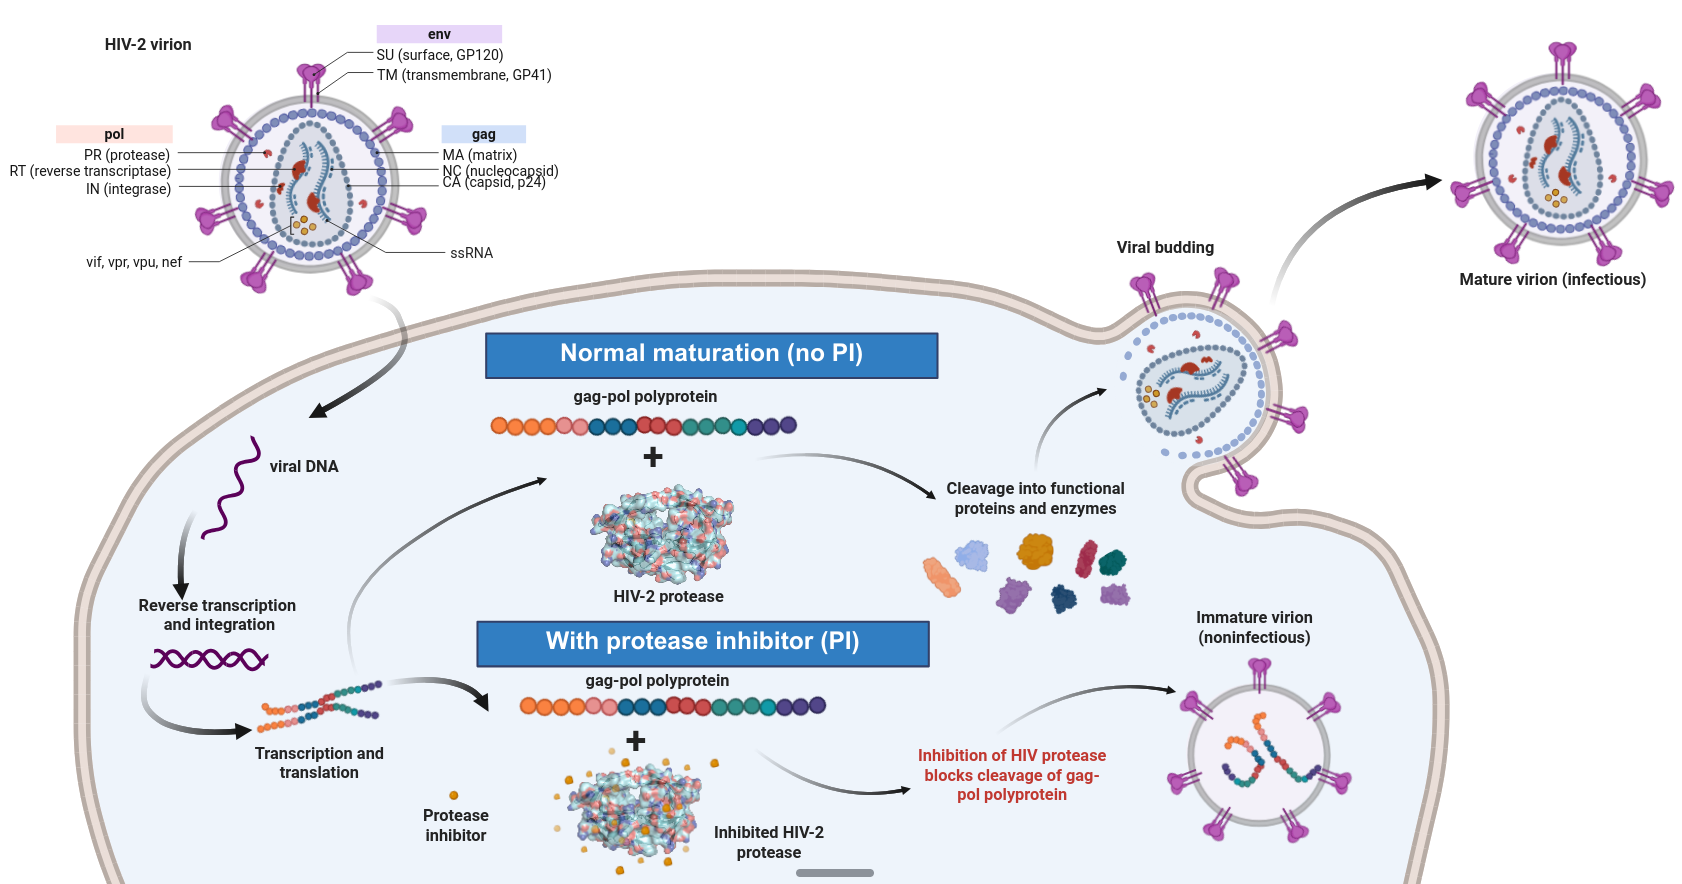
\includegraphics[width=\linewidth]{Figures/Maturation_Inhibition.png}
		\caption{Schéma du rôle de la protéase dans la maturation du VIH2. Inhibiteur de protéase (\textit{protease inhibitor}) empêche les clivages des polyprotéines.}
		\label{fig:hiv2_maturation}
	\end{figure}
	\newpage
	\begin{wrapfigure}{r}{0.66\textwidth} 
		\centering
		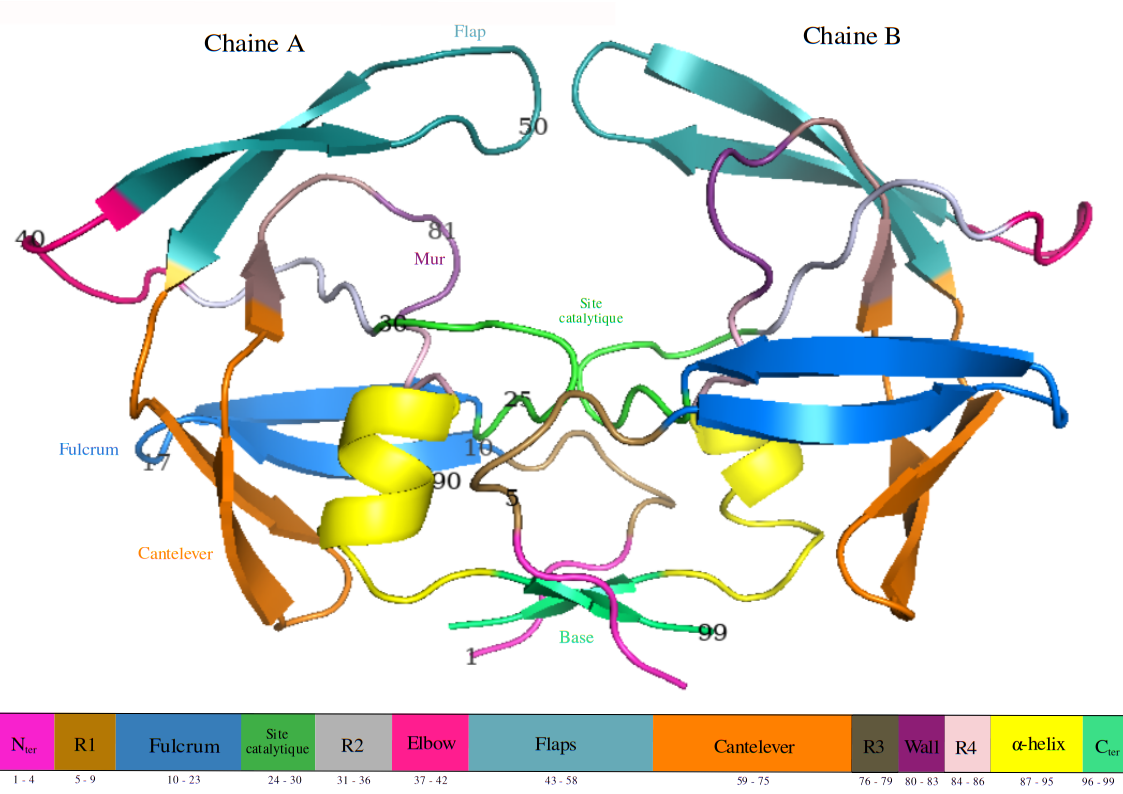
\includegraphics[width=\linewidth]{Figures/PR2_structure_1.png}
		\caption{La structure tridimensionnelle de la protéase dimère VIH-2. Structure à partir d'entrée PDB 1HSI.}
		\label{fig:PR2_strct}
	\end{wrapfigure}
	La protéase permet la décomposition des protéines en unités protéiques plus petites, telles que les peptides ou les acides aminés. La protéase du VIH-2 est une protéase \textbf{aspartique}, qui assure la médiation des clivages protéolytiques des polyprotéines Gag et Gag-Pol pendant ou juste après la libération du virion de la membrane plasmatique, pour produire des protéines matures infectieuses (Fig.~\ref{fig:hiv2_maturation}). Les inhibiteurs -- soit du site actif, soit de la dimerisation -- empêchent le VIH de se répliquer. \\
	Structurellement, la protéase VIH-2 est un homodimère, composé de deux chaînes polyprotéiques structurellement identiques, constituées chacune de 99 acides aminés (Fig.~\ref{fig:PR2_strct}). Le site actif de la PR2 est formé à l'interface du dimère et contient deux résidus d'acide aspartique catalytique, chacun d'eux étant apporté par leur sous-unités respectives, pour former deux motifs Asp-Thr-Gly (résidus 25 à 27). Deux régions de volets (\textit{flaps}) flexibles identiques participent également à la liaison d'inhibiteurs et de substrats~\cite{scott_curling_2000}.\par
	Plus précisément, la flexibilité des \textit{flaps} permet à l'enzyme de se trouver en conformation ouverte, semi-ouvert ou fermé~\cite{chen_revealing_2014, sadiq_explicit_2010, hornak_hiv-1_2006}. À l'état semi-ouvert, les \textit{flaps} sont soulevés, ce que permet l'entrée de substrat vers le site actif. Lorsqu'un ligand se lie au site actif la PR2 passe d'une forme semi-ouverte à une forme fermée, qui permet de recouvrir le site actif avec ligand lié, et donc induit l'action catalytique. Il a été démontré également qu'au cours de changements conformationnels, les réarrangements au niveau des \textit{flaps}, plus précisément le passage d'un \textit{flap} de chaine B devant \textit{flap} de chaine A, permet la fermeture ultérieure~\cite{hornak_hiv-1_2006, baillif_2026_18495249}. \par
	De plus, il est connu que les inhibiteurs de PR1 cliniquement approuvés ciblent directement la dyade catalytique~\cite{kar_origin_2012}. Lorsque l'inhibiteur se lie au site catalytique, la dyade symétrique est transformée en dyade qui adopte un état de protonation asymétrique. Il est alors d'un grand intérêt d'étudier l'absence de ce proton (état déprotoné) afin de mieux comprendre l'effet que la protonation a sur les réarrangements conformationnels, ainsi que sur la dynamique d'ouverture ou de fermeture de la protéine.\par
	La question globale que nous nous sommes posés au cours de ce projet était :~\emph{Quelle est l'impact de la protonation sur le comportement dynamique de la protéase du VIH-2 (PR2)?}\\
	Plus précisément, l'objectif de ce stage consiste en analyse des simulations de dynamiques moléculaires afin de définir l'impact de l'état de monoprotonation du site catalytique (Asp25, chaîne B) sur la conformation protéique, ainsi que sur la flexibilité globale et locale de la PR2.\\
	
	
	\section{Matériels \& Méthodes}
	\subsection{Réalisation de Dynamique Moléculaire (DM)}
		\begin{wraptable}{r}{0.5\textwidth}
		\vspace{-10pt}
			\centering
		\begin{tabular}{@{}lll@{}}
			\toprule
			\textbf{Condition} & \textbf{Nom}  & \textbf{Tps de sim (ns)}  \\ \midrule
			Déprototoné (DP)   & V11          & 1 000       \\
			Déprototoné (DP)   & V12          & 1 000       \\
			Déprototoné (DP)   & V1           & 1 000       \\
			Monoprotoné (MP)   & V7           & 1 000       \\
			Monoprotoné (MP)   & V8           & 500         \\
			Monoprotoné (MP)   & V21          & 500         
		\end{tabular}
		\caption{Tableau récapitulant les 6 simulations étudiés et ses conditions}
		\label{tab:simulations}
	\end{wraptable}
	Afin de répondre à notre question d'étude, on a pris l'un des structures existantes pour PR2. Ici, on s'est base sur l'entree PDB 1HSI (PR2 non complexée à un inhibiteur (forme apo), résolution de 1.9 \AA). Elle a été utilisé comme structure de départ pour la DM. Les six simulations ont été lancées à partir de cette structure en utilisant différentes 
	conditions de simulations : 3 en conditions déprotoné (V7,V8,V21) et 3 en conditions monoprotoné (V1,V11,V12), résume en tableur~\ref{tab:simulations}.
	
	
	L'hydrogène rajouté pour les DM en conditions MP se trouve au niveau de carbone-$\delta$ d'Aspartate 25 de la chaine B (Fig.~\ref{fig:protonation}), et essaie d'imiter les conditions de protonation lors d'une introduction d'inhibiteur de protéase. 
	
	\begin{figure}[h]
		\centering
		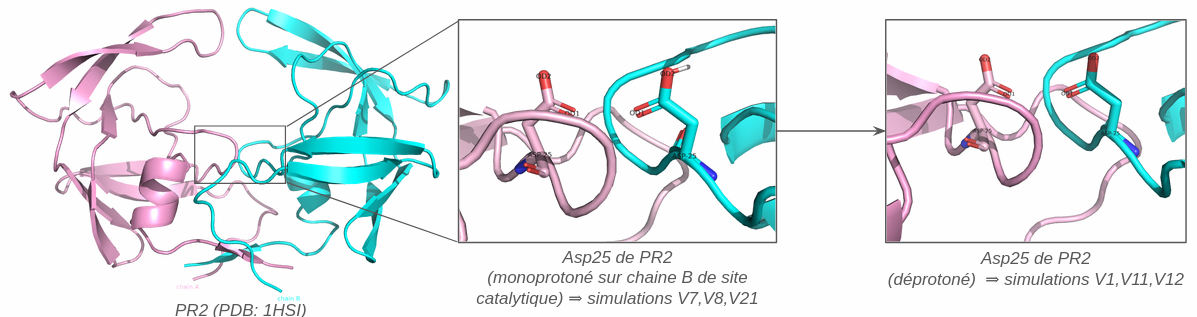
\includegraphics[width=1\linewidth]{Figures/protonation_on_1HSI.png}
		\caption{Visualisation de la structure monoprotoné (utilisé pour V7,V8,V21) et déprotoné (utilisé pour V1,V11, V12).}
		\label{fig:protonation}        
	\end{figure}
	
	Les simulations de DM ont été effectuées hors de ce stage et le protocole peut être retrouvée en Annexes (\ref{A1}). Les résultats des simulations ont été analysés visuellement en VMD, ainsi que numériquement en Python (packages \lstinline{MDAnalysis}, \lstinline{MDtraj}) et R (package  \lstinline{bio3D}). Les codes développés pendant ce stage sont tous accessibles sur \href{https://github.com/annhater/M1_STAGE}{GitHub}.
	
	\subsection{Métriques d'Analyse Structurale}
	\subsubsection{$\text{RMSD}_{\text{stepwise}}$}
	Tout au début, afin de faire une premiere evaluation des changements structurels causes par protonation, on voulait comparer la stabilité du système au cours de différentes simulations.
	Pour cela, il est d’intérêt d'utiliser la métrique de RMSD (\textit{Root Mean Square Deviation}), qui permet de mesurer la distance entre les atomes des molécules superposées. La formule de RMSD peut être retrouvé en Annexes(\ref{A2}). Dans notre cas, on compare la conformation de la protéine au moment $x$ contre la structure de la simulation entière moyenné.
	%Les deux valeurs ont été calculées avec les fonctions \lstinline{rms} et \lstinline{align} du package \lstinline{MDAnalysis.analysis} afin de calculer la structure "moyenne" (\textit{average structure}) au cours de toute la simulation, qui a été aligné sur le squelette protéique (\textit{backbones}).
	Pour valeurs de RMSD, les carbones $\alpha$ de chaque frame de simulation a été aligné sur les carbones $\alpha$ de frame 0 (structure de départ).
	
	\subsubsection{RMSF}
	Lorsqu'on a défini comment la structure évolue au cours de temps, on voudrais preciser quels sont les résidus qui sont impliques dans changement conformationnel.
	Pour cela, la métrique de RMSF (\textit{Root Mean Square Fluctuation}) a été calculé. Elle permet de mesurer l'écart de la position d'une particule (dans notre cas les carbones $\alpha$) par rapport à une position de référence (position d'atome moyenne) dans le temps.
	La formule pour calculer les valeurs de RMSF, peut être retrouve en Annexes (\ref{A3}).
	
	\subsubsection{Distances inter-résidus}
	Par la suite, lorsqu'on a défini les résidus lesquels on voudrait observer plus en detail au cours de simulations, on a d'abord analysé les distances entre ces résidus d’intérêt.
	La matrice des distances (qui considère toutes les paires des atomes en fonction des frames) a été crée avec le logiciel GROMACS.
	Depuis cette matrice, on a pu extraire les distances $d_{50-50}$, $d_{25-25}$, $d_{25-50}$, $d_{17-40}$.
	%De plus, pour l'analyse des distances intra-atomiques plus précises entre les atomes OD1 et OD2 d'Asp25 de chaine A avec OD2 d'Asp25 de la chaine B (sur laquelle agit la protonation), on a utilisé \lstinline{MDAnalysis.analysis.distances} (cf. \lstinline{02_analysis_ASP_OD.py}).
	
	\subsubsection{Projection de résidu 50 de la chaîne B sur le plan défini par les résidus 49, 50, et 51 de la chaîne A}
	Au cours de notre analyse, il était d’intérêt de regarder la dynamiques des \textit{flaps}, qui joue un role importante dans la conformation finale.
	Pour cela, on a applique la métrique de projection de résidu 50 de la chaîne B sur le plan défini par les résidus 49, 50, et 51 de la chaîne A ($d_{50B\xrightarrow{}49-50A-51A}$).
	Cette métrique développé par mes encadrantes, Dr. Lesie Regad et Mme Marine Baillif permet de quantifier le déplacement de \textit{flap} B par rapport au \textit{flap} A (le long de la perpendiculaire au plan du \textit{flap}).
	La valeur negative de cette métrique indique que \textit{flap} A se trouve devant \textit{flap} B, la conformation qui est observé dans les cas classiques dans la literature. La valeur positive indique sur \textit{flap} B qui se trouve devant \textit{flap} A, conformation laquelle on appel "inverse" par la suite.
	

	\subsubsection{$\text{RMSD}_{\text{pairs}}$}
	La MD V12 (DP) s'est révélé un intérêt particulière pour nous, puisque le système se refermait dans une meme manière comme les simulations en conditions DP (cf.Résultats).
	Pour définir les similitudes qu'on observe entre ces simulations, on a calcule le $\text{RMSD}_{\text{pairs}}$. Similaire au $\text{RMSD}_{\text{stepwise}}$, elle calcule la la distance entre les atomes des molécules superposées.
	Par contre, ici, on calcule cette distance entre chaque frame de simulation V12 et simulation V7, laquelle on a pris comme reference de simulations MP. Comme ça, on a construit une matrice carre de distances RMSD (\ref{A4}, Fig.~\ref{fig:pw_RMSD}), et observé les similitudes et differences des movements atomiques par paires de frames.
	
	\subsubsection{Distance de Jaccard}
	D'une manière similaire au $\text{RMSD}_{\text{pairs}}$, on a calculé la distance de Jaccard, qui permet de mesurer la similarité entre deux ensembles d'objets (Eq.\ref{eq:jaccard}).
	Dans notre cas, les objets sont les liaisons hydrogènes qui se forment au cours de simulation.
	
	\begin{equation}{}
		{\displaystyle J(A,B)={\frac {|A\cap B|}{|A\cup B|}}={\frac {|A\cap B|}{|A|+|B|-|A\cap B|}}}
		\label{eq:jaccard}
	\end{equation}
	

	\subsection{Analyse multivariée}
	\subsubsection{Classification hiérarchique}
	Les deux métrique précédentes ont était utilisé par la suite pour construire une dendrogramme, qui regroupe les frames de ces deux simulations en fonction de leur distances (méthode multivarie qui est aussi appelé regroupement hiérarchique ou hclust).
	\subsubsection{Construction d'une arbre de décision}
	En utilisant les liaisons hydrogènes qui se forment au cours de simulation, on a construit une matrice binaire (présence ou absence de liaison), qui a été filtré selon la variance entre les deux phases (phase 1 et phase 2).
	Cette matrice a été utilisé pour construire un arbre de décision, qui permet d'identifier les liaisons les plus importantes pour différencier les deux phases.
	
	
	\section{Résultats}
	%L'hypothèse de départ, qui s'est formé après l'observation de 6 simulations de dynamiques moléculaires, reposait sur le fait qu'en condition de monoprotonation sur Asp25 de la chaine B (MP) la conformation finale est fermée et stable pour toutes les simulations réplicats (V7,V8,V21).
	%On suppose que la fermeture est assurée par des liaisons fortes entre les aspartates de dyade.
	%Cependant, les simulations en conditions déprotonées ont révélé trois comportements conformationnels différents : conformations ouvertes (V11), fermée standard (V12), ou fermée inversée (V1), ce qui indique que la protonation n'est pas obligatoire pour la fermeture.
	%Ce projet vise donc à identifier les réseaux d'interactions moléculaires précis qui gouvernent ces mécanismes de repliement et de stabilisation alternative. 
	%Pour ce faire, nous avons réalisé une analyse bio-informatique en utilisant Python et R pour calculer les métriques de distance ($d_{50-50}$, $d_{25-50}$, $d_{17-40}$), ainsi qu'appliqué la métrique de trajectoires qui existaient déjà, comme RMSD, RMSF et la projection $d_{50B\xrightarrow{}49-50A-51A}$ (développés par mes tutrices, Mme Marine Baillif au cours de sa thèse et Mme Leslie Regad).
	
	Dans le but de répondre au question globale de ce projet, on a réalisé un analyse consecutif des DM en différentes conditions.
	D'abord, on a défini les changements conformationnels globaux qui se produisent au cours de simulation, ainsi que les régions de la protéine qui sont impliquées dans ces changements. Par la suite, on a analysé les interactions moléculaires qui se forment autour le site catalytique, et qui peuvent être impliquées dans la stabilisation de la conformation fermée.
	Enfin, on a appliqué des méthodes de classification hiérarchique pour identifier les événements structuraux discrets qui accompagnent la stabilisation de la structure de PR2 (1HSI).
	Les détails sur les métriques utilisées sont présentés auparavant, ar la suite on analysera les résultats de ceux les plus pertinents.

	\subsection{Etude de la dynamique globale de la PR2 selon l'état de protonation}
	L'analyse de la dynamique globale de la protéine au cours de simulation nous a permis de observer les changements conformationnels qui se produisent au cours de simulation.
	Les valeurs de la métrique $\text{RMSD}_{\text{stepwise}}$, nous a permis d'observer les differences globales qui se produisent au cours de simulation et les differences entre les deux conditions de protonation.
	Grace à cette étude, nous avons observé que les valeurs de RMSD varie beaucoup plus pour les simulations déprotonés, sauf V12, qui ressemble les simulations MP (Fig.~\ref{fig:RMSD}).
	Analyse RMSD nous a permis d'également préciser le moment de stabilisation de la structure. On a décidé d'appeler le période de système instable, qui échantillonne toutes les conformations différentes, la phase 1 (ou $\phi_1$); lorsque le système se stabilise et reste dans une conformation jusqu'à la fin de la simulation, il entre dans la phase 2 ($\phi_2$).
	Comme ça on a défini les frames-limites de la phase 1 pour toutes les simulations (sauf pour V11, qui reste ouverte et donc toujours en $\phi_1$): V7 = 198, V8 = 180, V21 = 155, V12 = 35, V1 = 517.
	
	\begin{figure}[h]
		\centering
		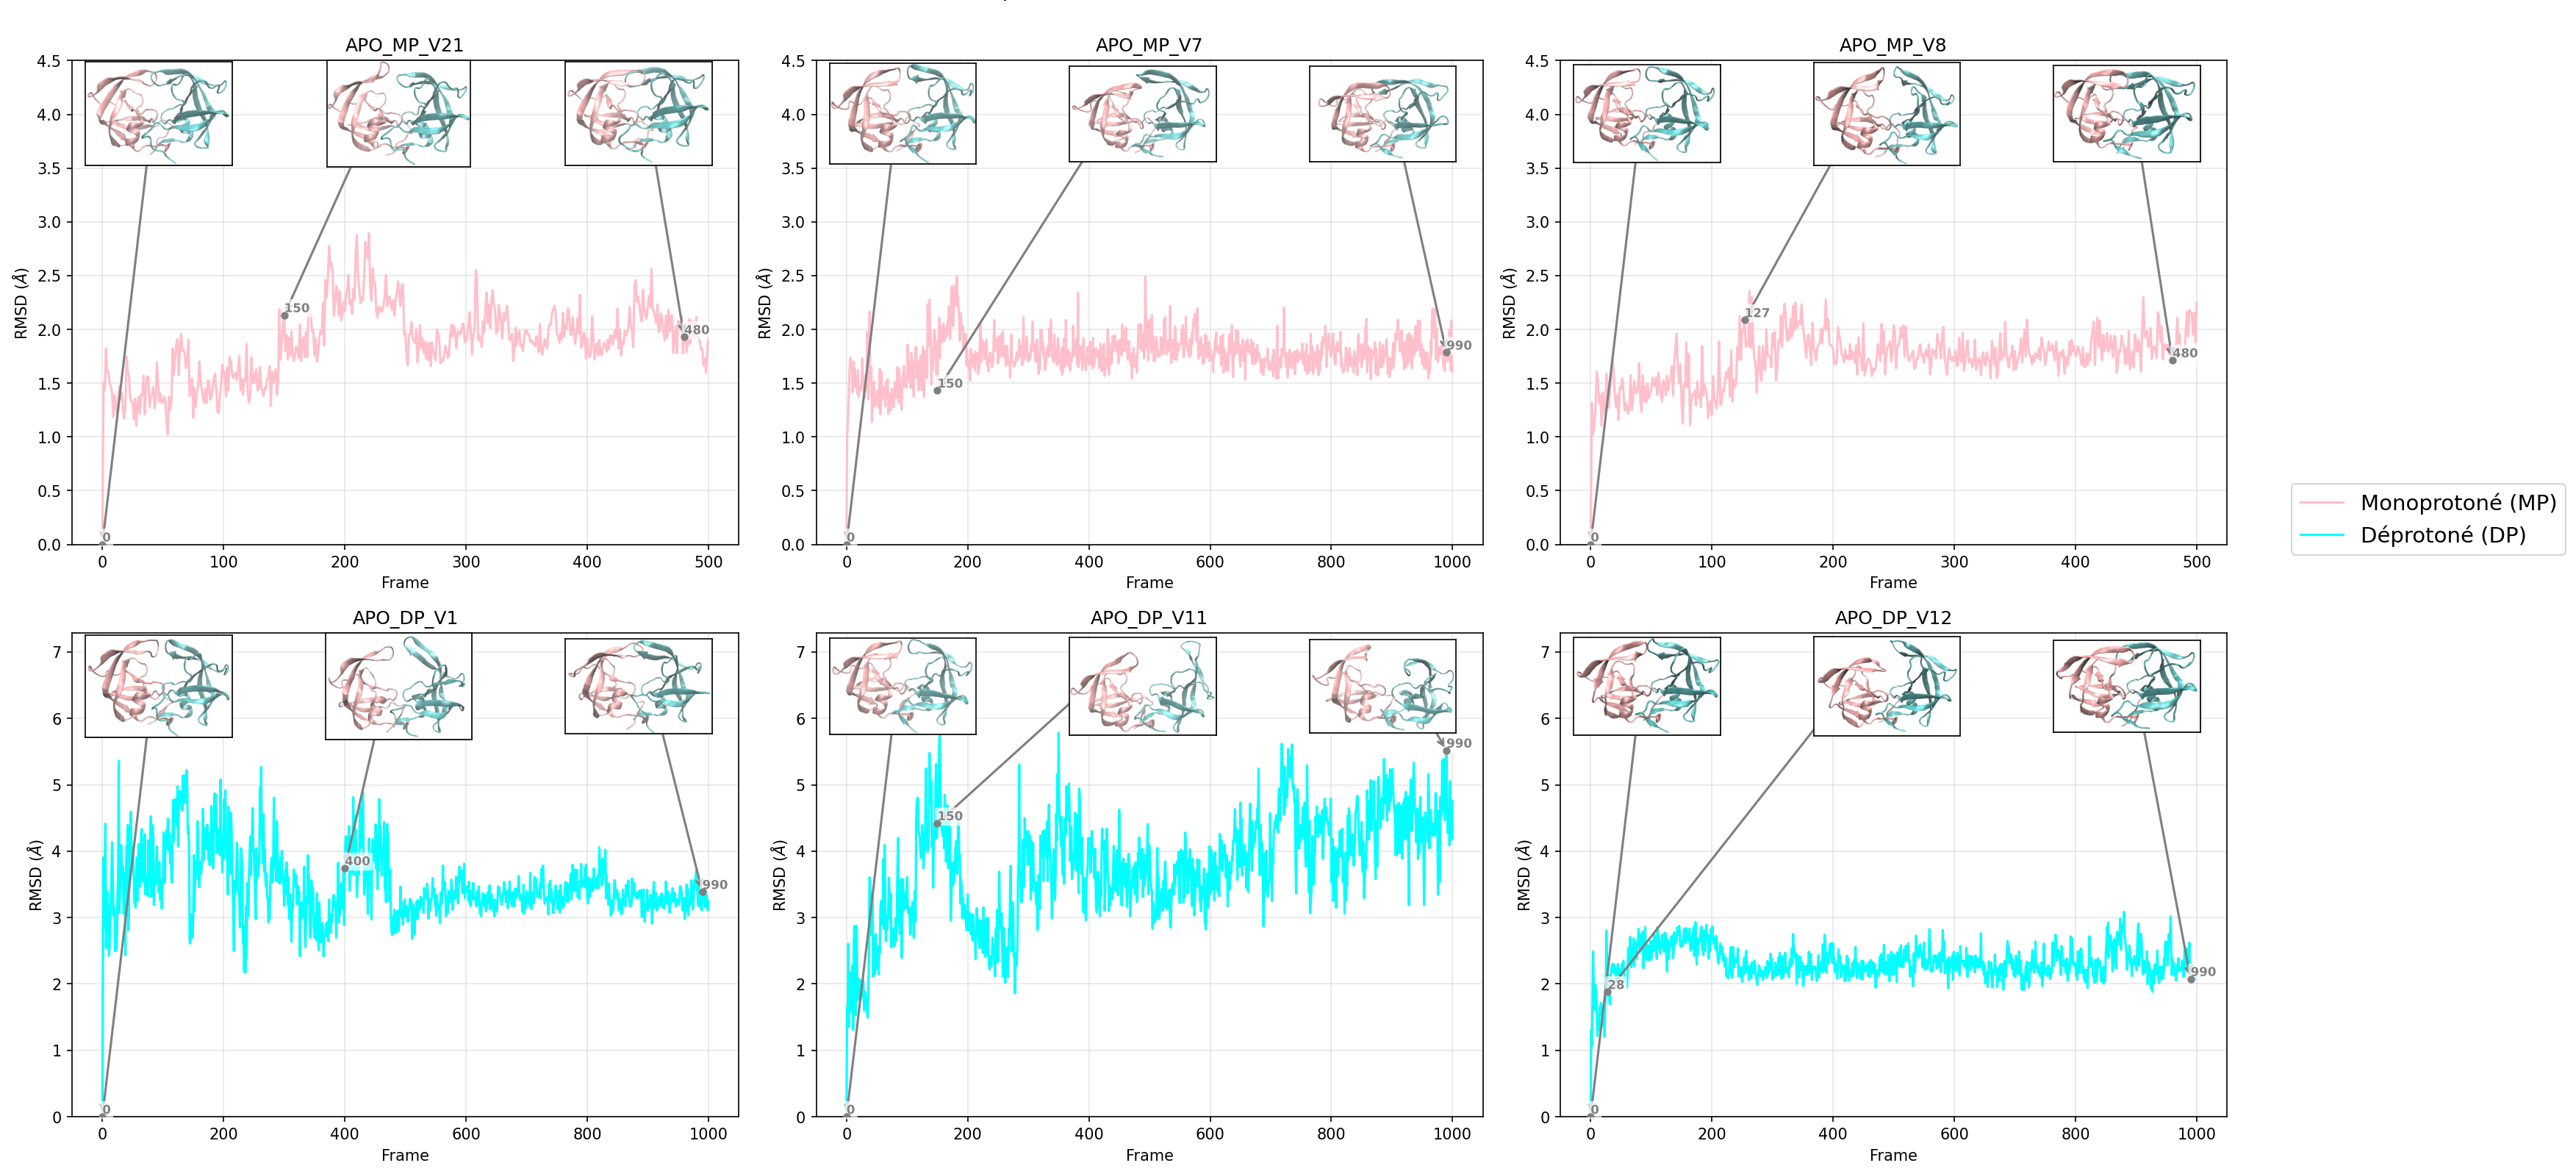
\includegraphics[width=\linewidth]{Figures/rmsd_steps_w_frames_unscaled.png}
		\caption{Analyse $\text{RMSD}_{\text{stepwise}}$ (fluctuation moyenne quadratique de chaque frame par rapport au structure initiale) entre les six simulations étudiées. RMSD calculé sur les carbones $\alpha$.}
		\label{fig:RMSD}
	\end{figure}
	
	\subsection{Etude de flexibilité de la PR2 selon l'état de protonation} \label{sec:RMSF}
	\begin{wrapfigure}{r}{0.5\linewidth}
		\centering
		%\vspace{-10pt}
		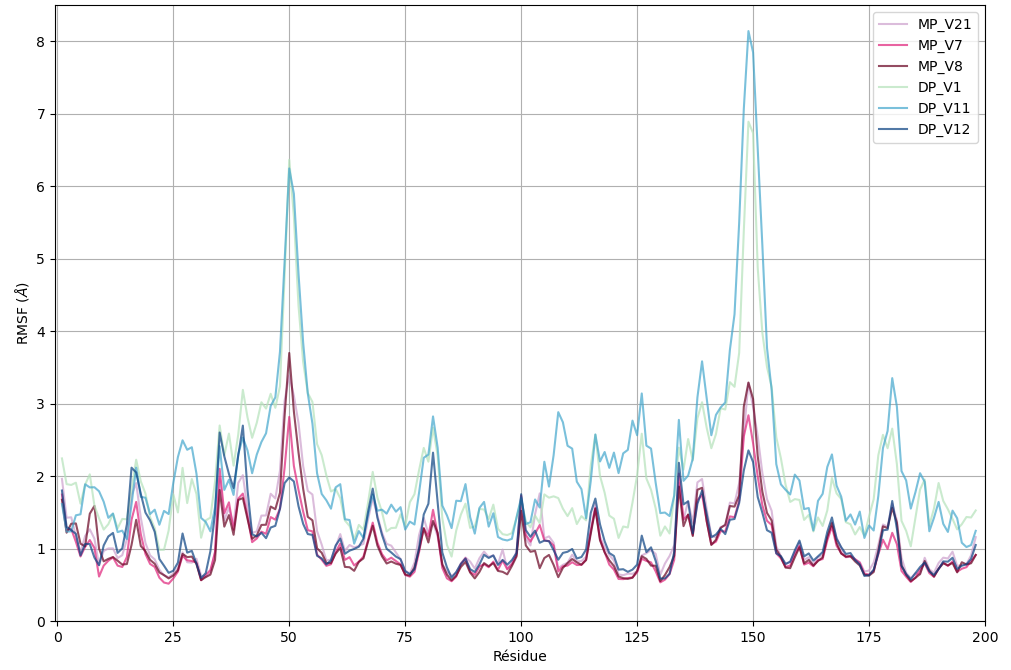
\includegraphics[width=\linewidth]{Figures/rmsf.png}
		\caption{Analyse RMSF (fluctuation moyenne quadratique) entre les six simulations étudiées. RMSF calculé sur les carbones $\alpha$, après un ajustement sur le squelette protéique.}
		\label{fig:RMSF}
	\end{wrapfigure}
	Par la suite, on voulait préciser quel est l'impact de la protonation sur la flexibilité de la structure et quels sont les résidus les plus mobiles au cours de simulation.
	Pour cela, on a fait une analyse de RMSF, qui permet d'accéder aux variances des positions atomiques au cours de simulation (Fig.~\ref{fig:RMSF}).
	Nos résultats ont démontré qu'on peut regrouper le comportement en deux catégories. L'un, c'est fermeture "classique", qui démontre une flexibilité peu élevée (entre valeurs de 0.5 à 4.5), avec les simulations monoprotonés: V7, V8, V21, et V12 (déprotoné, néanmoins, se ferme avec \textit{flap} A devant \textit{flap} B).
	L'autre cas, plus "flexible", avec des valeurs RMSF plus élevées (de 1 à 8 \AA), avec V11 qui se trouve en conformation ouverte et V1 qui est ferme dans une manière inverse, avec \textit{flap} B devant \textit{flap} A.
	De plus, on a observé des pics de flexibilité autours les résidus 50 et 149 (\textit{flaps}), pour toutes les simulations, ce que est en accord avec literature, qui indiste sur l'importance des flaps dans la conformation finale.
	Pour les les V1 et V11 on observe des pics de flexibilité autours des résidus 25-30 (site catalytique), qui peuvent expliquer les différences de comportement observées.
	%On a pu conclure que la monoprotonation toujours stabilise le système et cause la fermeture avec \textit{flap} A devant \textit{flap} B, par contre, la déprotonation cause un comportement imprévisible : si le système peut se stabiliser au cours de simulation, la protéine se ferme d'une manière stable et peu flexible, comme pour V12, sinon, le système reste très flexible au cours de simulation.
	
	\subsection{Caractérisation géométrique des régions d'intérêt}
	Les résultats d'etude de la dynamique globale et de flexibilité nous a permis de définir les régions d'intérêt pour l'analyse plus détaillée, qui sont : les résidus 25-30 (site catalytique), les résidus 50-51 (flaps), les résidus 17-40 (région de la boucle supérieure).
	Cela nous a amené de continuer vers analyse de variation des distances entre les résidus d'interet.
	Après l'analyse des métriques de distances pour les chaines A et B (\ref{A4}, Figs.~\ref{fig:d25_50_chA},\ref{fig:d25_50_chB},\ref{fig:d25_25},\ref{fig:d50}), on fait des conclusions similaires qu'avant : la séparation de phases est visible, avec phase 1 qui échantillonne des distances intra-atomiques différentes et puis se stabilise dans la phase 2 ($d_{50-50}$ autours 7-9 \AA, $d_{25-25}$ autours 5-7 \AA, $d_{25-50}$ autours 14-16 \AA). De plus, ces métriques sont plus élevées pour les simulations V1 et V11, où on observe les conformations flexibles, ce que confirme encore une fois que dans ces simulations, à cause de déprotonation, on n'a pas réussi de former un système stable au niveau du site catalytique.
	
	\subsection{Analyse de la dynamique des flaps : la projection $d_{50B\xrightarrow{}49-50A-51A}$}
	Vu l'importance de la dynamique des flaps dans la conformation finale, qu'on a identifié auparavant, on a appliqué la métrique de projection $d_{50B\xrightarrow{}49-50A-51A}$, pour démontrer le lien entre conformation de flaps et stabilisation de la structure finale.
	On a observé que pour V1, lors de la stabilisation (517 ns) la position des \textit{flaps} est inversée (\textit{flap} B devant \textit{flap} A) (Fig.~\ref{fig:d50_projection}). Cela suggere que pour la fermeture de flaps, le rearrangement de flaps n'est pas nécessaire.
	Par contre, pour atteindre une conformation stable au niveau du site catalytique (comme on a vu en Section \ref{sec:RMSF}), la fermeture de flaps correcte (A devant B) est nécessaire. 
	\begin{figure}
		\centering
		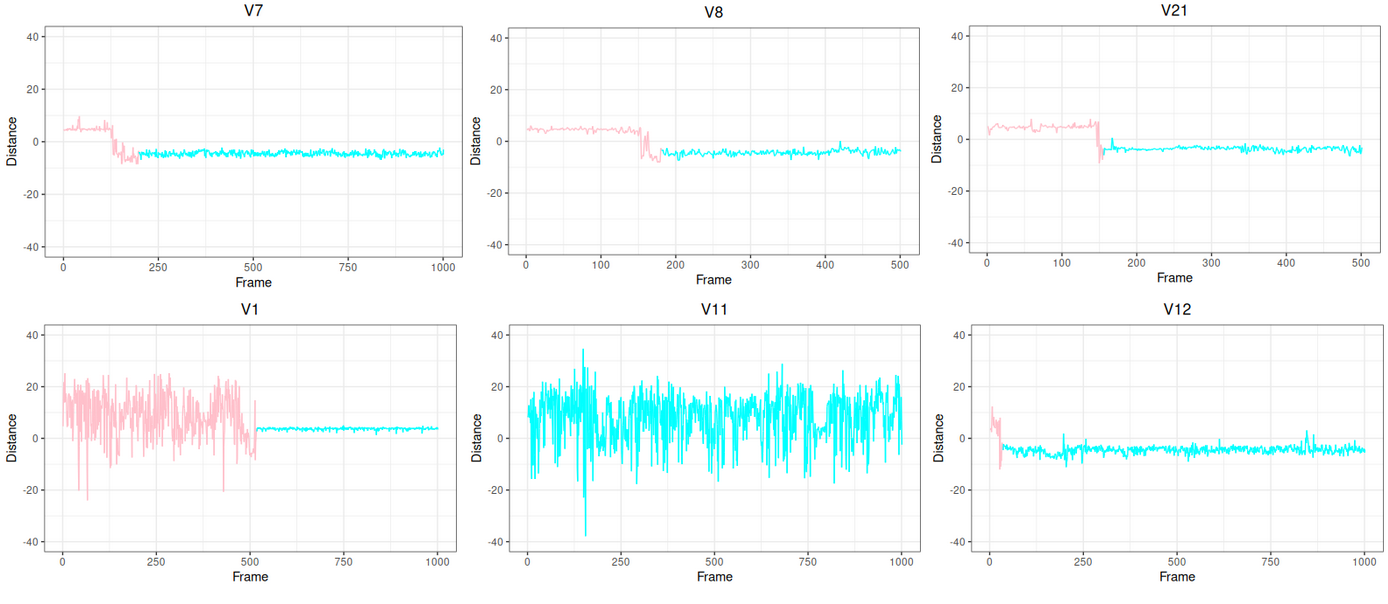
\includegraphics[width=0.9\linewidth]{Figures/d50_projection.png}
		\caption{Analyse de la projection $d_{50B\xrightarrow{}49-50A-51A}$ pour les six simulations : MP (V7,V8,V21) et DP (V1,V11,V12). Une valeur de projection négative indique que le \textit{flap} A est devant \textit{flap} B, alors qu'une valeur positive indique l'inversion des \textit{flaps}. Phase 1 (phase flexible) est coloré en rose, phase 2 (phase de stabilisation) est coloré en cyan.}
		\label{fig:d50_projection}
	\end{figure}
	
	\subsection{Analyse d'environnement du site catalytique : les réseaux d'interactions} \label{sec:interactions}
	%wrap figure on the next page, to avoid the problem of figure placement
	
	Comme on a identifie l'effet que la protonation a sur le mouvement des flaps et stabilisation du site catalytique, il etait d'interet pour nous d'analyser plus en detail les interactions qui se forment autour du site catalytique et de voir s'il y a un correlation entre formation des liasons stabilisantes et stabilisation du système avec arrangement des flaps correcte.
	En analysant les liaisons autour le site catalytique (Fig.~\ref{fig:interaction_heatmap}), on note la différence globale qui est dans l'interaction de dyade Asp25-Asp25, et interactions avec Arg8 (de R1), Arg87 (d’hélice $\alpha$).
	Grace au comportement de V12 similaire aux MP, on note des interactions possiblement stabilisantes : Asp25-Gly27, Asp25-Thr26, Asp25-Thr26, Asp25-Gly27, Leu24-Leu97.
	
	\begin{wrapfigure}[23]{r}{0.33\textwidth}
		\centering
		%\vspace{-10pt}
		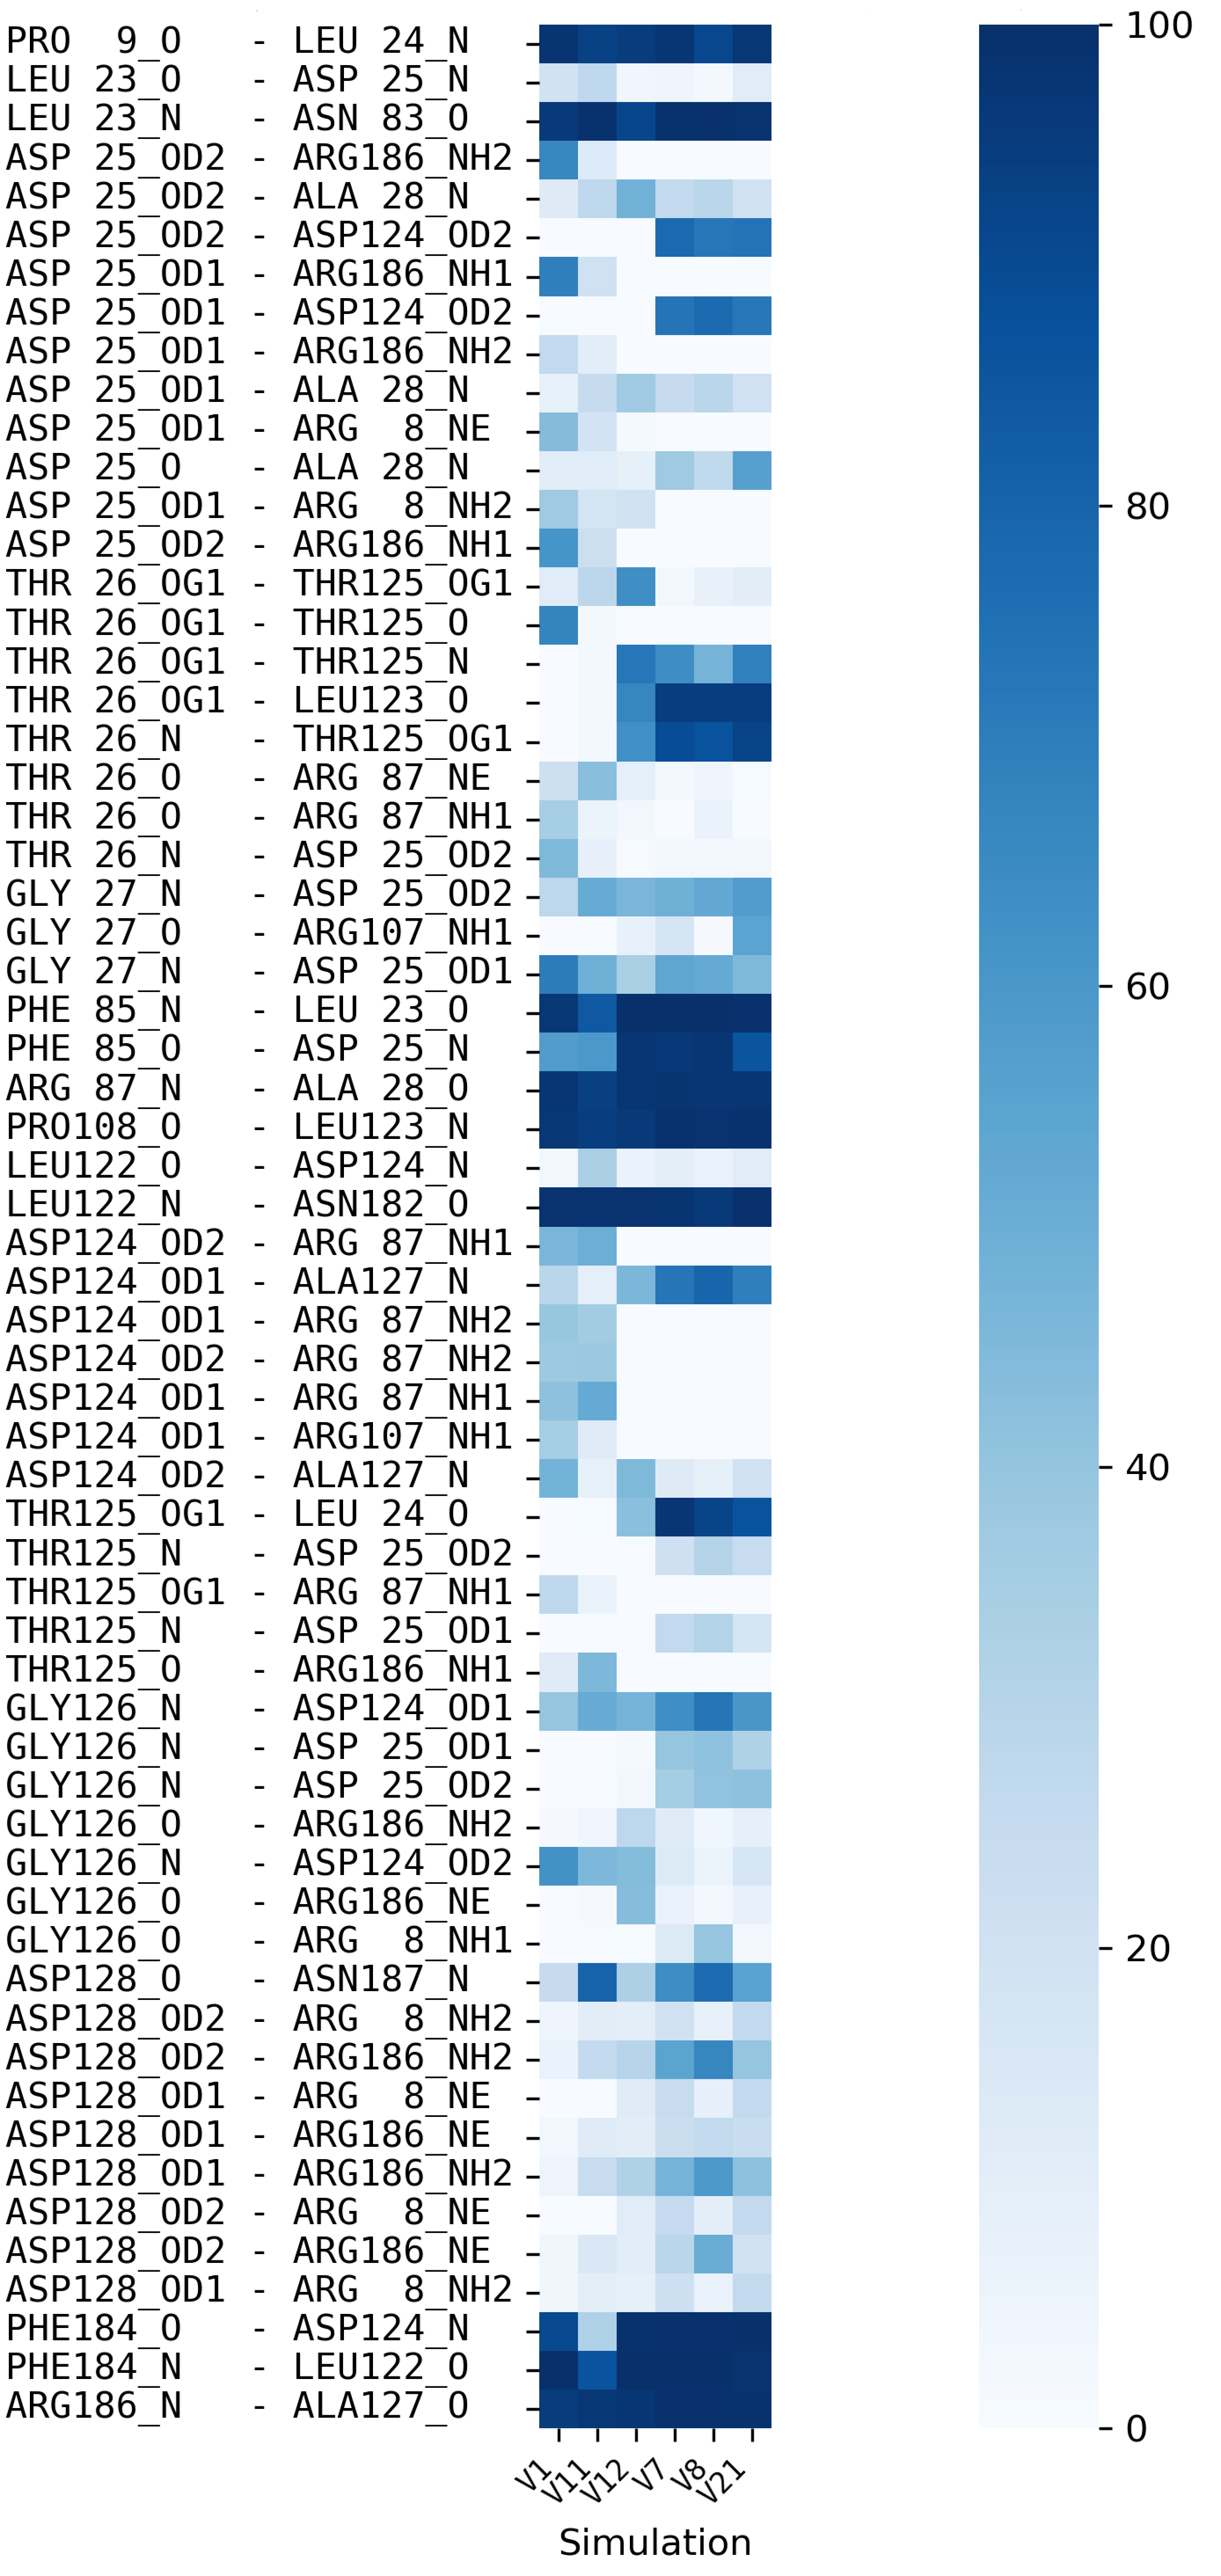
\includegraphics[width=\linewidth]{Figures/interactions_heatmap_2.png}
		\caption{Heatmap de fréquences d'interactions uniques qu'on retrouve autour le site catalytique (résidus 23, 24, 25, 26, 27, 28 de chaine A et B)} 
		\label{fig:interaction_heatmap}
	\end{wrapfigure}
	En comparant les fréquences les structures de différentes simulations, on note interaction Leu24-Val22, qui se forme. Pour V1, on note une interaction spécifique Thr26-Thr26 (\textit{side-chain to backbone}), ainsi que la région de R1 (résidus 5-9), qui s’approche plus fréquemment au site catalytique.
	On peut supposer que ces interactions peuvent être impliquées dans la stabilisation de la conformation fermée, et que l'absence de ces interactions peut expliquer le comportement plus flexible de V1 et V11.
	%Il est possible qu'il y a le fait de remplissage de l'espace vide laissé par les volets décalés.
	%Rajouter un reseau d'interactions pour les simulations (to do)
	
	
	\subsection{Analyse multivariée: classification hiérarchique}
	Afin de définir des règles possibles qui peuvent expliquer la stabilisation de la conformation fermée correcte dans le cas de deprotonantion (lequel on observe en V12), on a appliqué des méthodes d'analyse multivariée.
	Le but était de determiner quels sont les événements structuraux discrets qui differencient la phase 1 de la phase 2, et qui accompagnent la stabilisation de la structure de protéase.
	Pour cela on a pris deux simulations qui se sont stabilisées dans une conformation fermée (V7 et V12), mais qui sont en conditions differetes de protonation.
	L'analyse de $\text{RMSD}_{\text{pairs}}$ suivi par la construction d'une dendrogramme qui regroupe les frames de chaque simulation, n'a pas permis d'identifier de regrouppement de phases differrentes de chaque simulation (\ref{A4}, Fig.~\ref{fig:dendro_RMSD}).
	Cela indique sur le fait qu'au niveaux de mouvements dans la systeme la phase 1 de V7 ne resemble pas aux mouvements de phase 1 de V12.\\
	Comme on a observe presedement en partie~\ref{sec:interactions}, c'est possible que les similitudes en evenements permissives au stabilisation en forme correcte se trouvent au niveau des interactions.
	C'est pourquoi par la suite on s'est interessé de trouver les interactions communs en appliquant la distance de Jaccard au moment de transition entre deux phases.
	Grace aux plusieurs étapes de filtrage, on a identifie 67 interactions de haute variance entre phase 1 et phase 2, qui peuvent expliquer ce passage d'une phase instable à phase stabilisé. Là aussi, le regroupement n'a pas révélé un clusterisation par phases, mais plutot par simulations.  

\subsection{Analyse multivariée: l'arbre de décision}
Les résultats inconclusifs de classification hiérarchique nous ont menés à essayer un autre type d'analyse multivariée : l'arbre de décision (aussi parfois appelé CART, pour \textit{Classification and Regression Tree}).
Cette modèle se base sur la matrice binaire de présence/absence des liaisons hydrogènes de haute variance qu'on a identifiée auparavant.
L'arbre de décision résultant est présenté dans la (Fig.\ref{fig:decision_tree_bonds}).
Le nœud racine de l'arbre isole l'interaction impliquant la liaison hydrogène $\text{ARG\_8\_NH1}$-$\text{GLY\_126\_O}$ situé entre les régions R1 et le site catalytique.
\newpage
\begin{wrapfigure}{r}{0.66\textwidth}
	\centering
    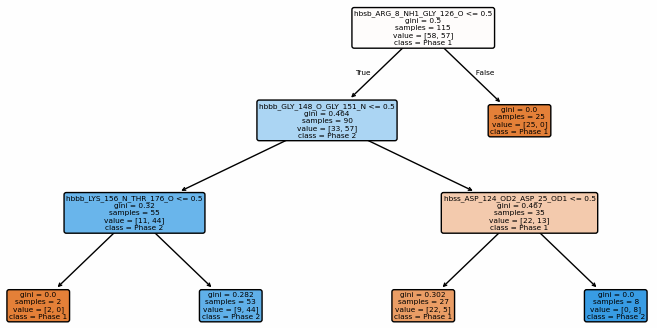
\includegraphics[width=\linewidth]{Figures/decision_tree_bonds.png}
    \caption{Arbre de décision développé selon les liaisons hydrogènes présentes V7/V12}
	\label{fig:decision_tree_bonds}
\end{wrapfigure}
L'absence de ce contact oriente majoritairement le tri vers la Phase 2, signifiant qu'une rupture locale ou un basculement de l'ancrage des résidus de la boucle supérieure est le prérequis pour la conformation stable fermée de la PR2.
Les nœuds inférieurs, impliquant notamment $\text{GLY148\_O}$-$\text{GLY151\_N}$ au niveau des flaps, complètent le partitionnement. Il est évident que l'interaction $\text{ASP124\_OD2}$-$\text{ASP25\_OD1}$ est possible seulement en conditions MP, et donc ici spécifique pour V7.
Lors de la vérification du modèle sur l'échantillon test, on obtient de bonnes valeurs de précision ($\phi_{1}:0.83,~\phi_{2}:0.76$) et sensibilité ($\phi_{1}:0.71,~\phi_{2}:0.87$). Ceci indique qu'on arrive à bien séparer la Phase 1 de la Phase 2 dans les deux simulations, et qu'on nécessite seulement trois interactions clés pour les discriminer.
Ce modèle basé sur les interactions souligne ainsi les contacts d'intérêt qui peuvent expliquer le passage inter-phasique. En perspective, on pourrait développer ce modèle pour toutes les simulations afin de confirmer l'importance des interactions aux endroits identifiés.

\subsection{Étude de comportement du cœur proteique}
	D'apres les résultats d'analyse de l'environnement du site catalytique, on a identifié des interactions qui peuvent être impliquées dans la stabilisation de la conformation fermée, et que l'absence de ces interactions peut expliquer le comportement plus flexible de V1 et V11.
	\begin{figure}[h]
		\centering
		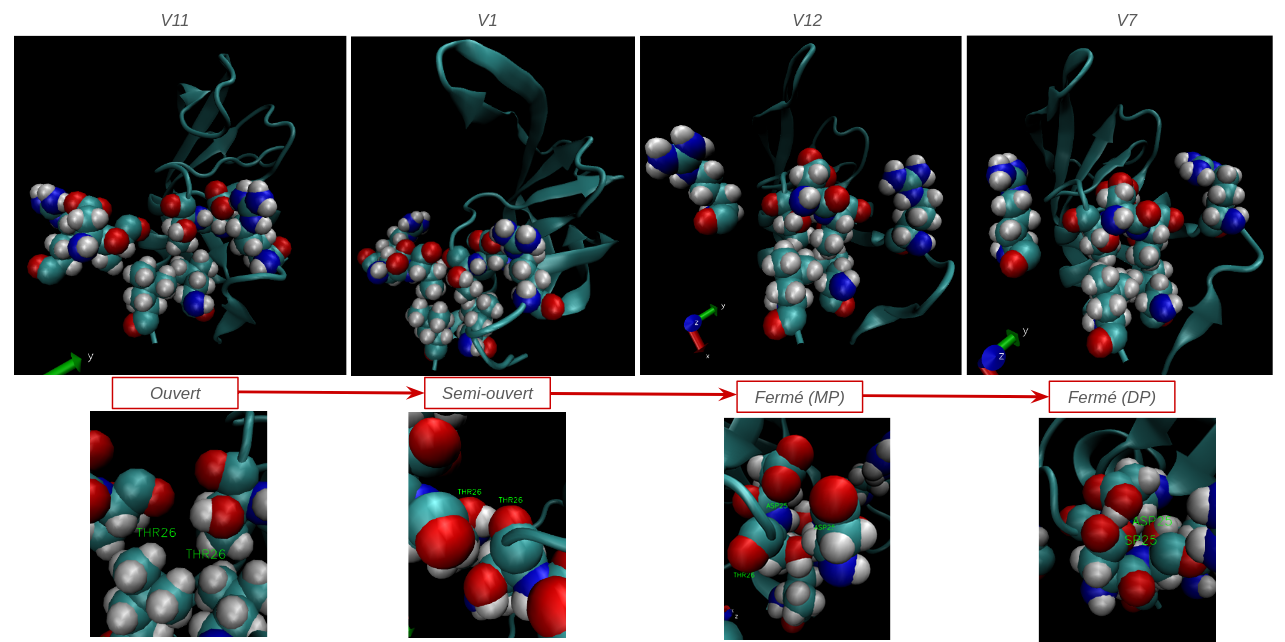
\includegraphics[width=\linewidth]{Figures/coeur_prot.png}
		\caption{Visualisation du cœur proteique en VMD pour les simulations V7, V12, V1 et V11. La stabilité de la structure finale est assurée par la formation d'un forte reseau d'interactions au niveau du cœur de la protéine, qui se forme autours le site catalytique.}
		\label{fig:coeur_prot}
	\end{figure}
	On a également proposé des régles moléculaires qui peuvent expliquer la stabilisation de la conformation fermée. Ce qu'on observe est que la phase 2, dans les simulations qui ont reussi de se stabiliser et fermer d'une manière classique, est caractérisé par la formation de liaisons hydrogènes entre les résidus du site catalytique et les résidus proches.
	En analysant le reseau d'interactions qui se forme autour le site catalytique au cours des simulations, on note la formation d'une interaction serrée et peut flexible autour du site catalytique.
	On peut faire des hypothèses que la formation d'une reseau stable, qui se ressemble à une bouchon (Fig.\ref{fig:coeur_prot}). Son absence dans V11 explique l’impossibilité de maintenir les flaps fermés avec arrangement des flaps correcte.
	
	
	\section{Discussion \& Conclusions}
	Au cours de ce projet de stage on s'est focalisé sur l'exploration des evenements qui sont à la base de la fermeture de la structure de la protéase PR2 (1HSI). Les dynamiques moléculaires réalisées en deux conditions -- monoprotoné et déprotoné -- nous a révélé trois types de structure finale possible: ouvert (V11), fermé avec le sens des flap A devant B et coeur protéique stable (V7,V8,V21,V12) et fermé mais avec flap B devant A et coeur protéique flexible.
	On a pu conclure que la monoprotonation toujours stabilise le système et cause la fermeture avec \textit{flap} A devant \textit{flap} B, par contre, la déprotonation cause un comportement imprévisible : si le système peut se stabiliser au cours de simulation, la protéine se ferme d'une manière stable et peu flexible, comme pour V12, sinon, le système reste très flexible au cours de simulation.
	Grace aux analyses d'environnement autour du site catalytique on a pu identifier des interactions qui jouent un role dans la stabilisation de la structure en conditions déprotonés, mais quel formation n'est pas assuré. On a identifié que la structure en V12 à réussi de se stabiliser grace à un réseau d'interactions
	
	\par En perspectives, on pourrait analyser espace 3D du site catalytique plus en detail, pour mettre en evidence la role d'un reseau d'interactions serré dans la fermeture correcte.
	De plus, on vise à construire une carte d'interactions au ce niveau là, pour voir si d'autres evemenements peuvent jouer un role dans stabilisation de la structure fermé.
	Cette étude indique sur un piste important dans dé le design d'inhibiteurs spécifiques au VIH-2 puisque il indique que meme en conditions de déprotonation, PR2 arrivé à se stabiliser et se fermer. Les médicaments ciblant la protéase doivent prendre cela en compte.
	
	\section{Remerciements}
	Ce stage de master a été effectué au sein d'équipe Profilage Pharmacologique In Silico (IsPP) de l'unité de Biologie Fonctionnelle et Adaptative (BFA) de l'Université Paris Cité, sous la direction de \textbf{Dr. Leslie Regad} et \textbf{Marine Baillif}, doctorante à IsPP, que je voudrais remercier pour proposition cette thématique vraiment intéressante, qui éclaire une vraie lacune en recherche de VIH. Je suis reconnaissante pour tous les conseils au cours de stage de l'organisation d'expériments à la rédaction de ce rapport. \par
	%J'adresse également ma reconnaissance chef d'équipe IsPP -- Dr. Pierre Tufféry, ainsi qu'au directeur de l’unité BFA Prof. Christophe Magnan, pour m’avoir donné l’opportunité de faire ce stage.
	%Les dessins du rapport ont été créés via \href{https://www.biorender.com/}{BioRender}. Les outils pour visualisation moléculaires sont PyMol~\cite{PyMOL} et VMD~\cite{HUMP96}.
	%Cette recherche a été menée à bien grâce à Université Paris Cité et Master Bio-Informatique -- In Silico Drug Design. 
	
	\newpage
	\addcontentsline{toc}{section}{Références}
	\bibliographystyle{unsrt} 
	\bibliography{masterBib} 
	\newpage
	
	\appendix
	\section{Annexes} \label{Annexes}
	
	\subsection{Protocole de simulations de dynamique moléculaire (DM)} \label{A1}
	Les simulations MD ont été effectuées avec GROMACS 2022 appliqué le champ de force AMBER99SB et mode TIP3P (au moins $1.0$ nm de solvant entre le soluté et bords de boîte). Neutralisation du système a été faite en ajoutant Na et Cl. Pour toutes les simulations, la minimisation était réalisée avec l'algorithme \textit{steepest descent} jusqu'à ce que la force maximale soit réduite en dessous de $1000$ $\text{kJ}\cdot\text{mol}^{-1}\cdot\text{nm}^{-1}$, avec un maximum de $50 000$ étapes de minimisation. L'équilibrage a été effectué en deux étapes : NVT (310 K, thermostat : V-rescale) et NPT (1 bar, barostat : Parrinello-Rahman).\\
	Les interactions électrostatiques à longue portée ont été traitées avec la méthode Particle Mesh Ewald (PME), en utilisant un espacement de grille de Fourier de 0,16 nm et d'interpolation de quatrième ordre. Les interactions Van der Waals et l'électrostatique à courte portée ont été calculés avec une coupure de 1,0 nm, et les interactions non liées ont été gérées à l'aide du schéma de coupure Verlet. Toutes les liaisons covalentes impliquant des atomes d'hydrogène ont été contraintes à l'aide de LINCS, permettant l'utilisation de l'étape de temps de 2 fs tout au long.\\
	L'étape de production, en conditions NPT (310 K, 1 bar) varie en durée pour les simulations : soit 1000 ns, soit 500 ns. Les coordonnées ont été sauvegardées toutes les 10 ps.
	
	\subsection{Formule de RMSD} \label{A2}
	
	\begin{equation}
		{\displaystyle {\begin{aligned}\mathrm {RMSD} (\mathbf {a} ,\mathbf {b} )& ={\sqrt {{\frac {1}{n}}\sum _{i=1}^{n}\|r_{i}(a)-r_{i}(b)\|^{2}}}
					\\ & n= \text{nombre d'atomes}
					\\ & \text{a et b} = \text{2 conformations différentes}
					\\ & r_{i}(a) = \text{vecteur position de l’atome i dans la conformation a}
					\\ & r_{i}(b) = \text{vecteur position de l’atome i dans la conformation b}
		\end{aligned}}}
		\label{eq:RMSD}    
	\end{equation}
	
	\subsection{Formule de RMSF} \label{A3}
	\begin{equation}
		{\displaystyle {\begin{aligned}\mathrm {RMSF}_i & ={\sqrt {{\frac {1}{nsteps}}\sum _{t=1}^{nsteps}\|r_{i}(t)-\langle r_{i}\rangle \|^{2}}}
					\\ & r_{i}(t) = \text{vecteur position de l’atome i au pas t}
					\\ & nsteps = \text{nombre de pas de simulation}
					\\ & \langle r_{i}\rangle = {\frac {1}{nsteps}}\sum _{t=1}^{nsteps} r_i(t) \text{ (positions atomiques moyennes)}
		\end{aligned}}}
		\label{eq:RMSF}    
	\end{equation}

	\subsection{Figures additionnelles} \label{A4}

	\begin{figure}[h]
		\centering
		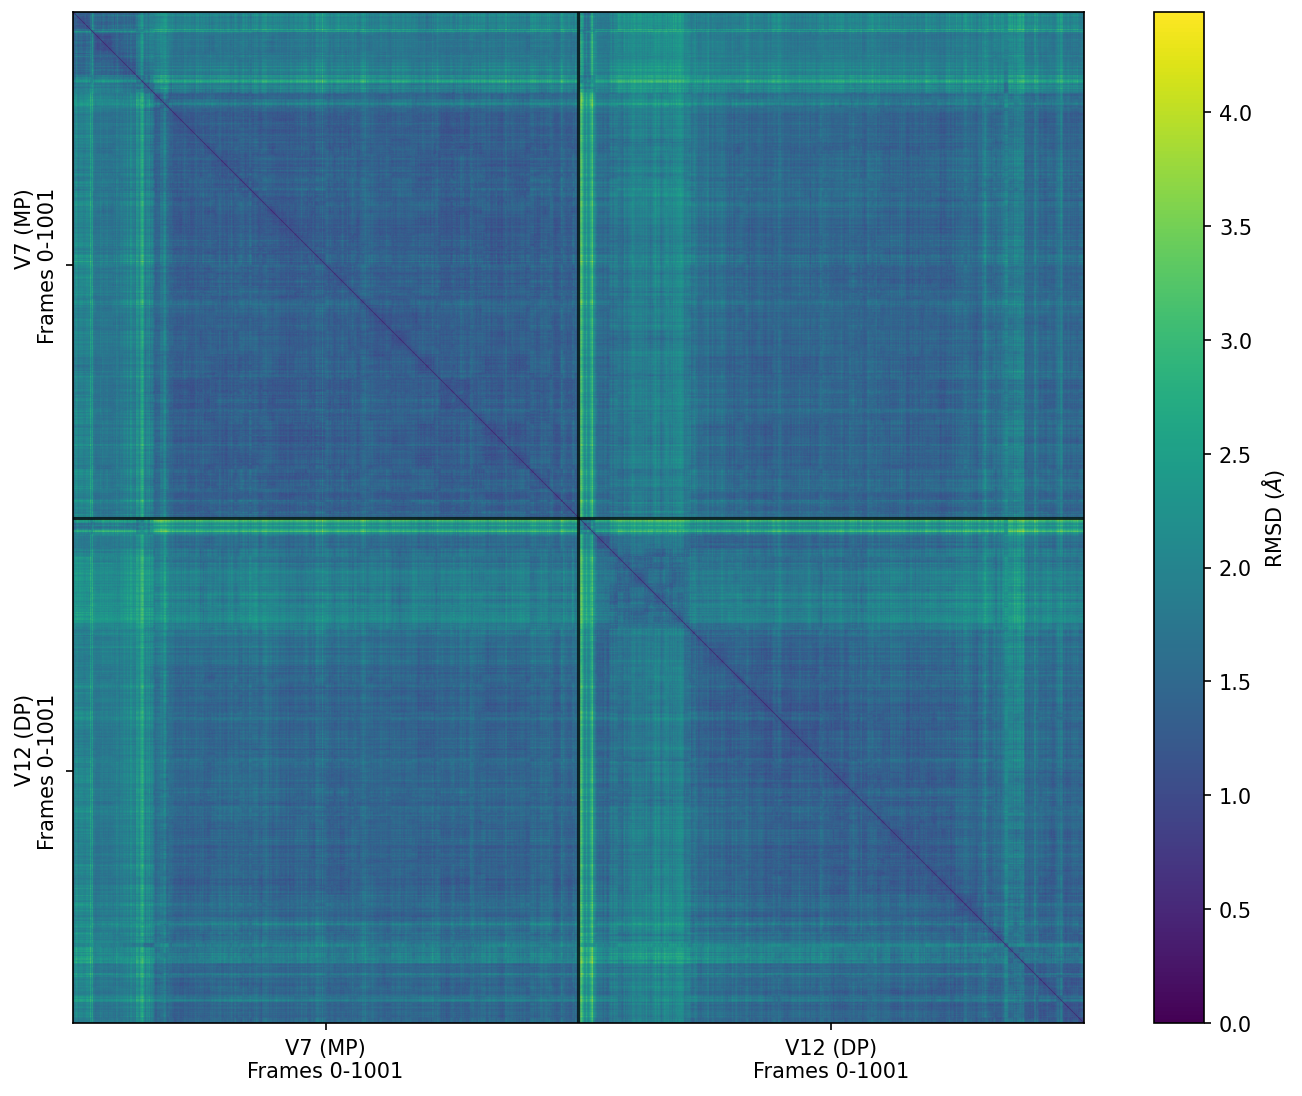
\includegraphics[width=0.66\linewidth]{Figures/pw_rmsd_V7_V12.png}
		\caption{Heatmap représentant la matrice de distances de RMSD par paires pour les deux simulations V7 (MP) et V12 (DP)}
		\label{fig:pw_RMSD}
	\end{figure}
	
	\begin{figure}[h]
		\centering
		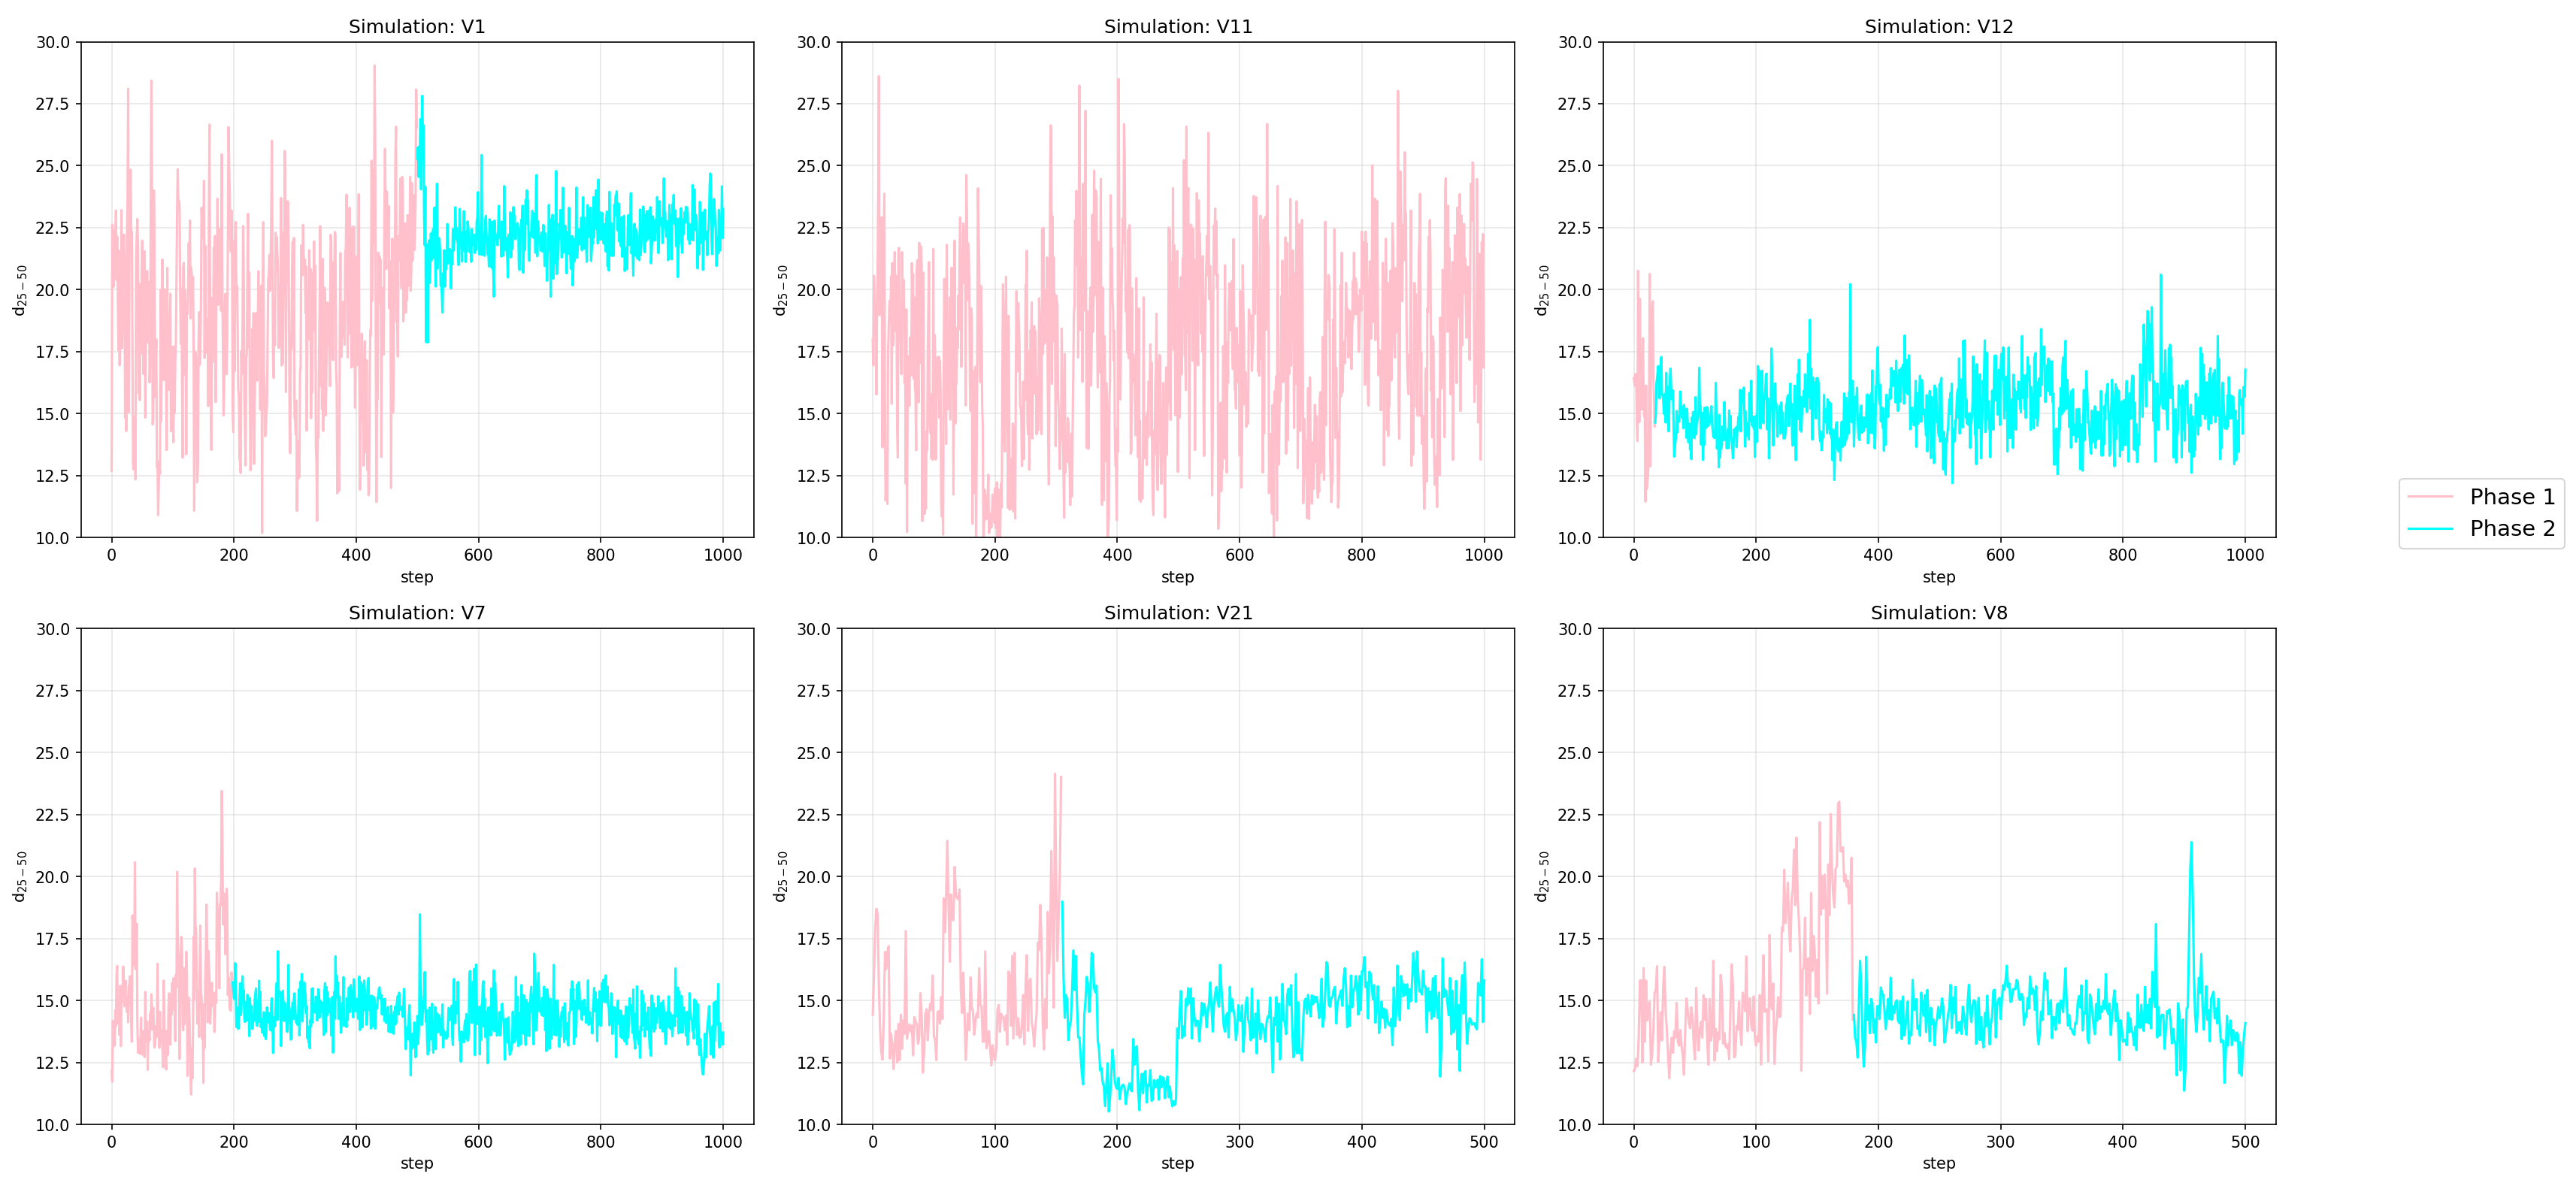
\includegraphics[width=\linewidth]{Figures/d_25_50_chA.png}
		\caption{Analyse $d_{25-50}$ la chaine A pour les six simulations : MP (V7,V8,V21) et DP (V1,V11,V12).}
		\label{fig:d25_50_chA}
	\end{figure}
	
	\begin{figure}[h]
		\centering
		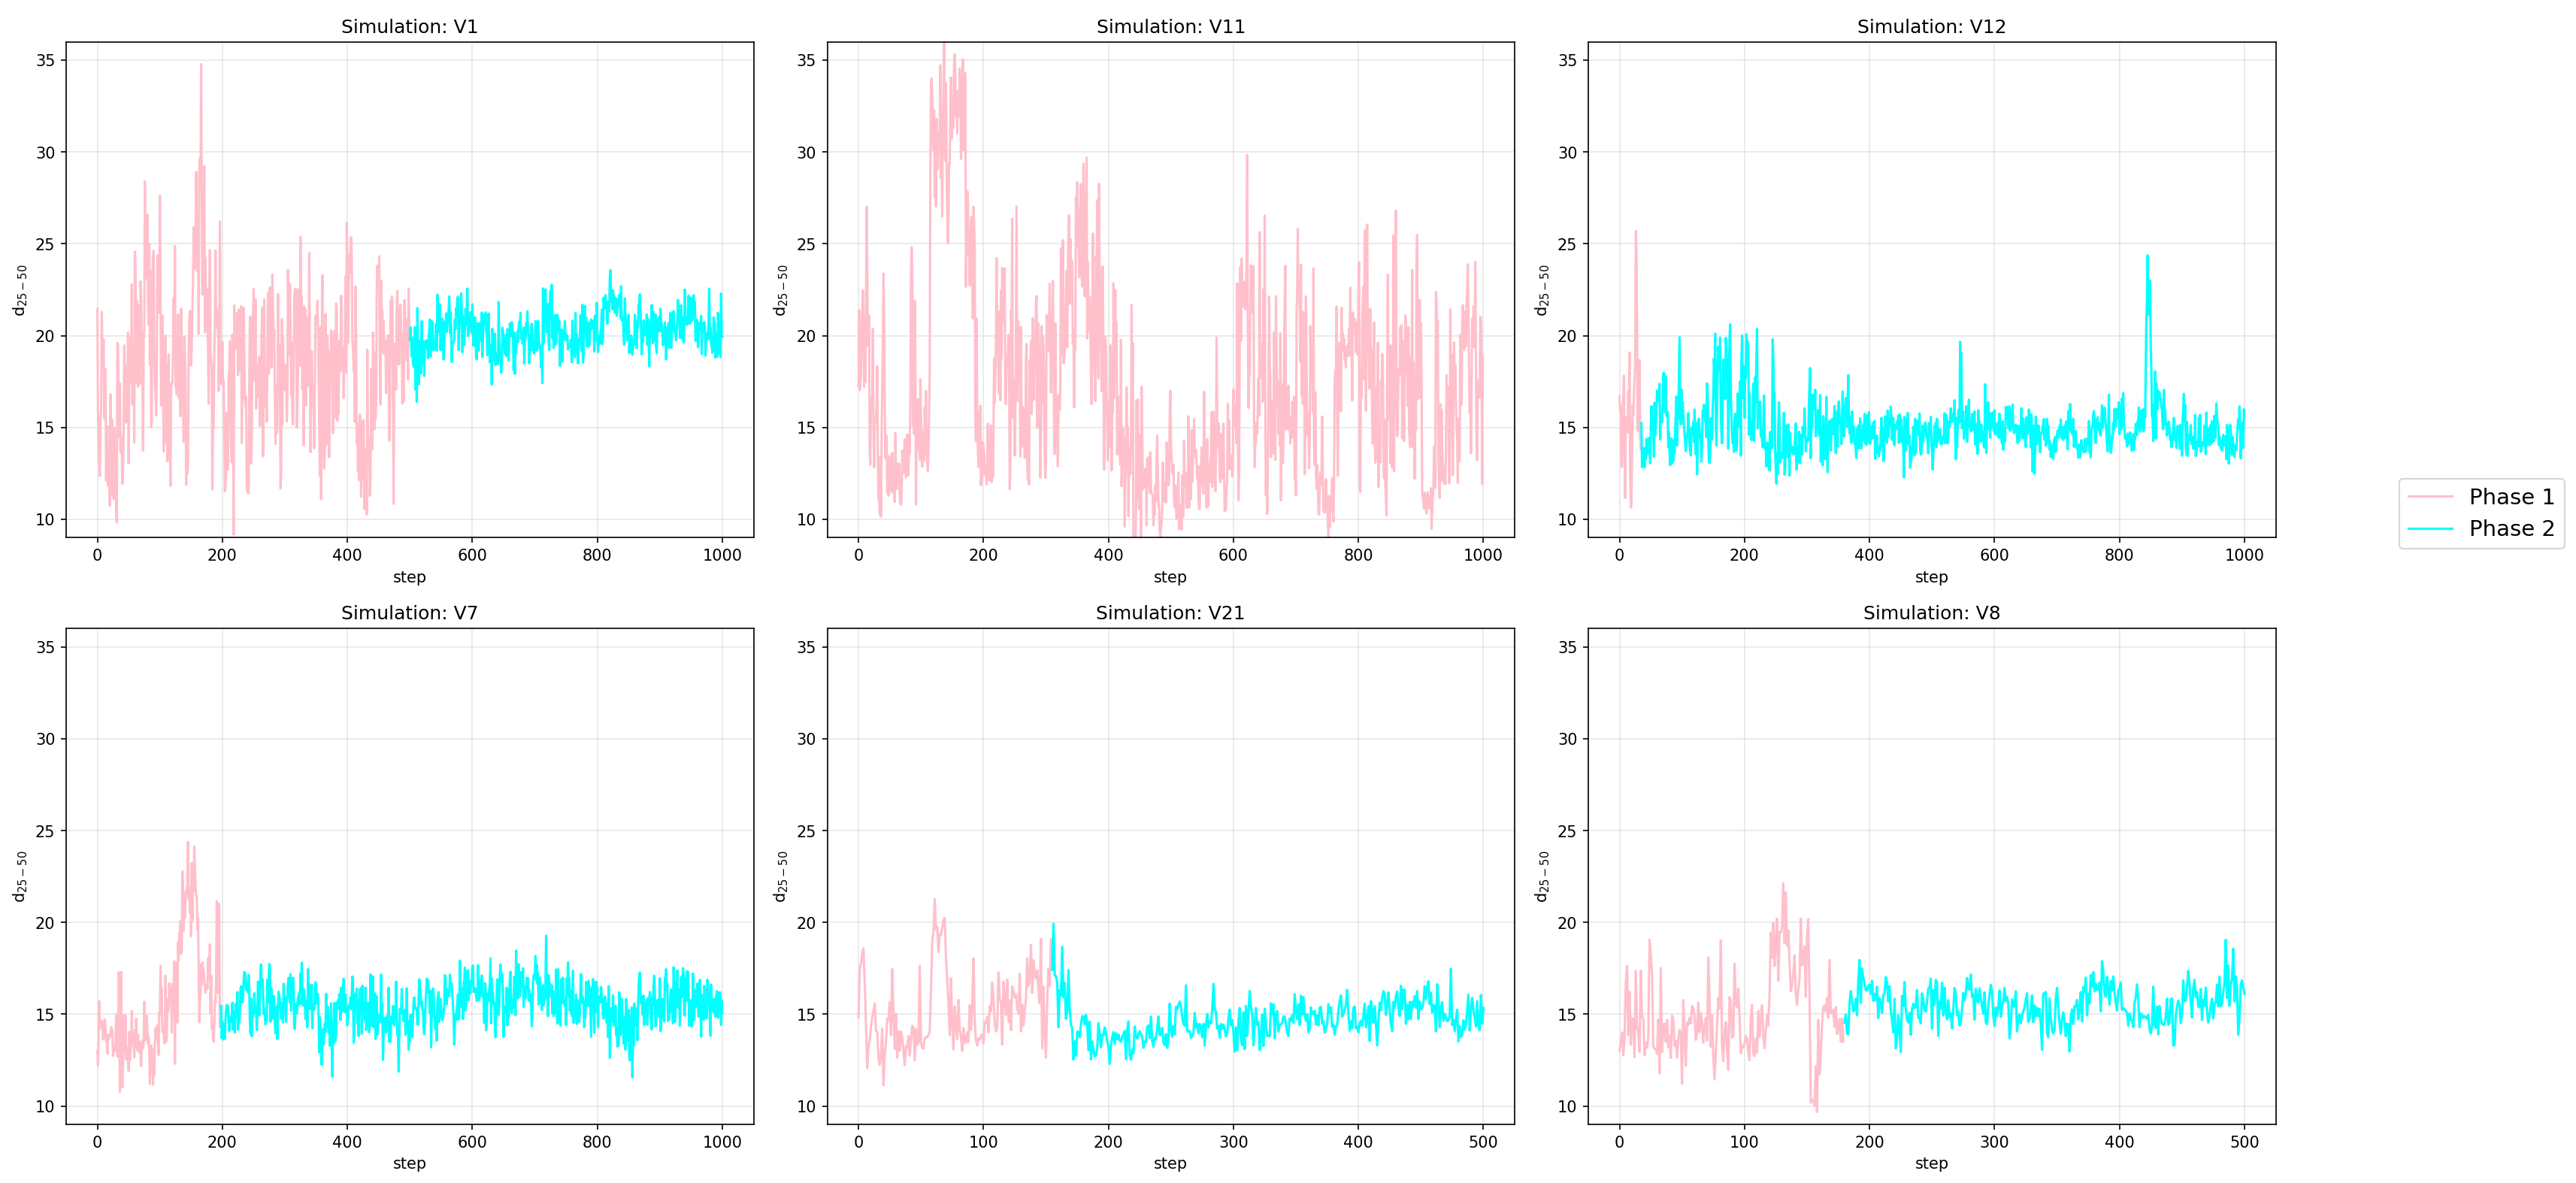
\includegraphics[width=\linewidth]{Figures/d_25_50_chB.png}
		\caption{Analyse $d_{25-50}$ la chaine B pour les six simulations : MP (V7,V8,V21) et DP (V1,V11,V12).}
		\label{fig:d25_50_chB}
	\end{figure}
	
	\begin{figure}[h]
		\centering
		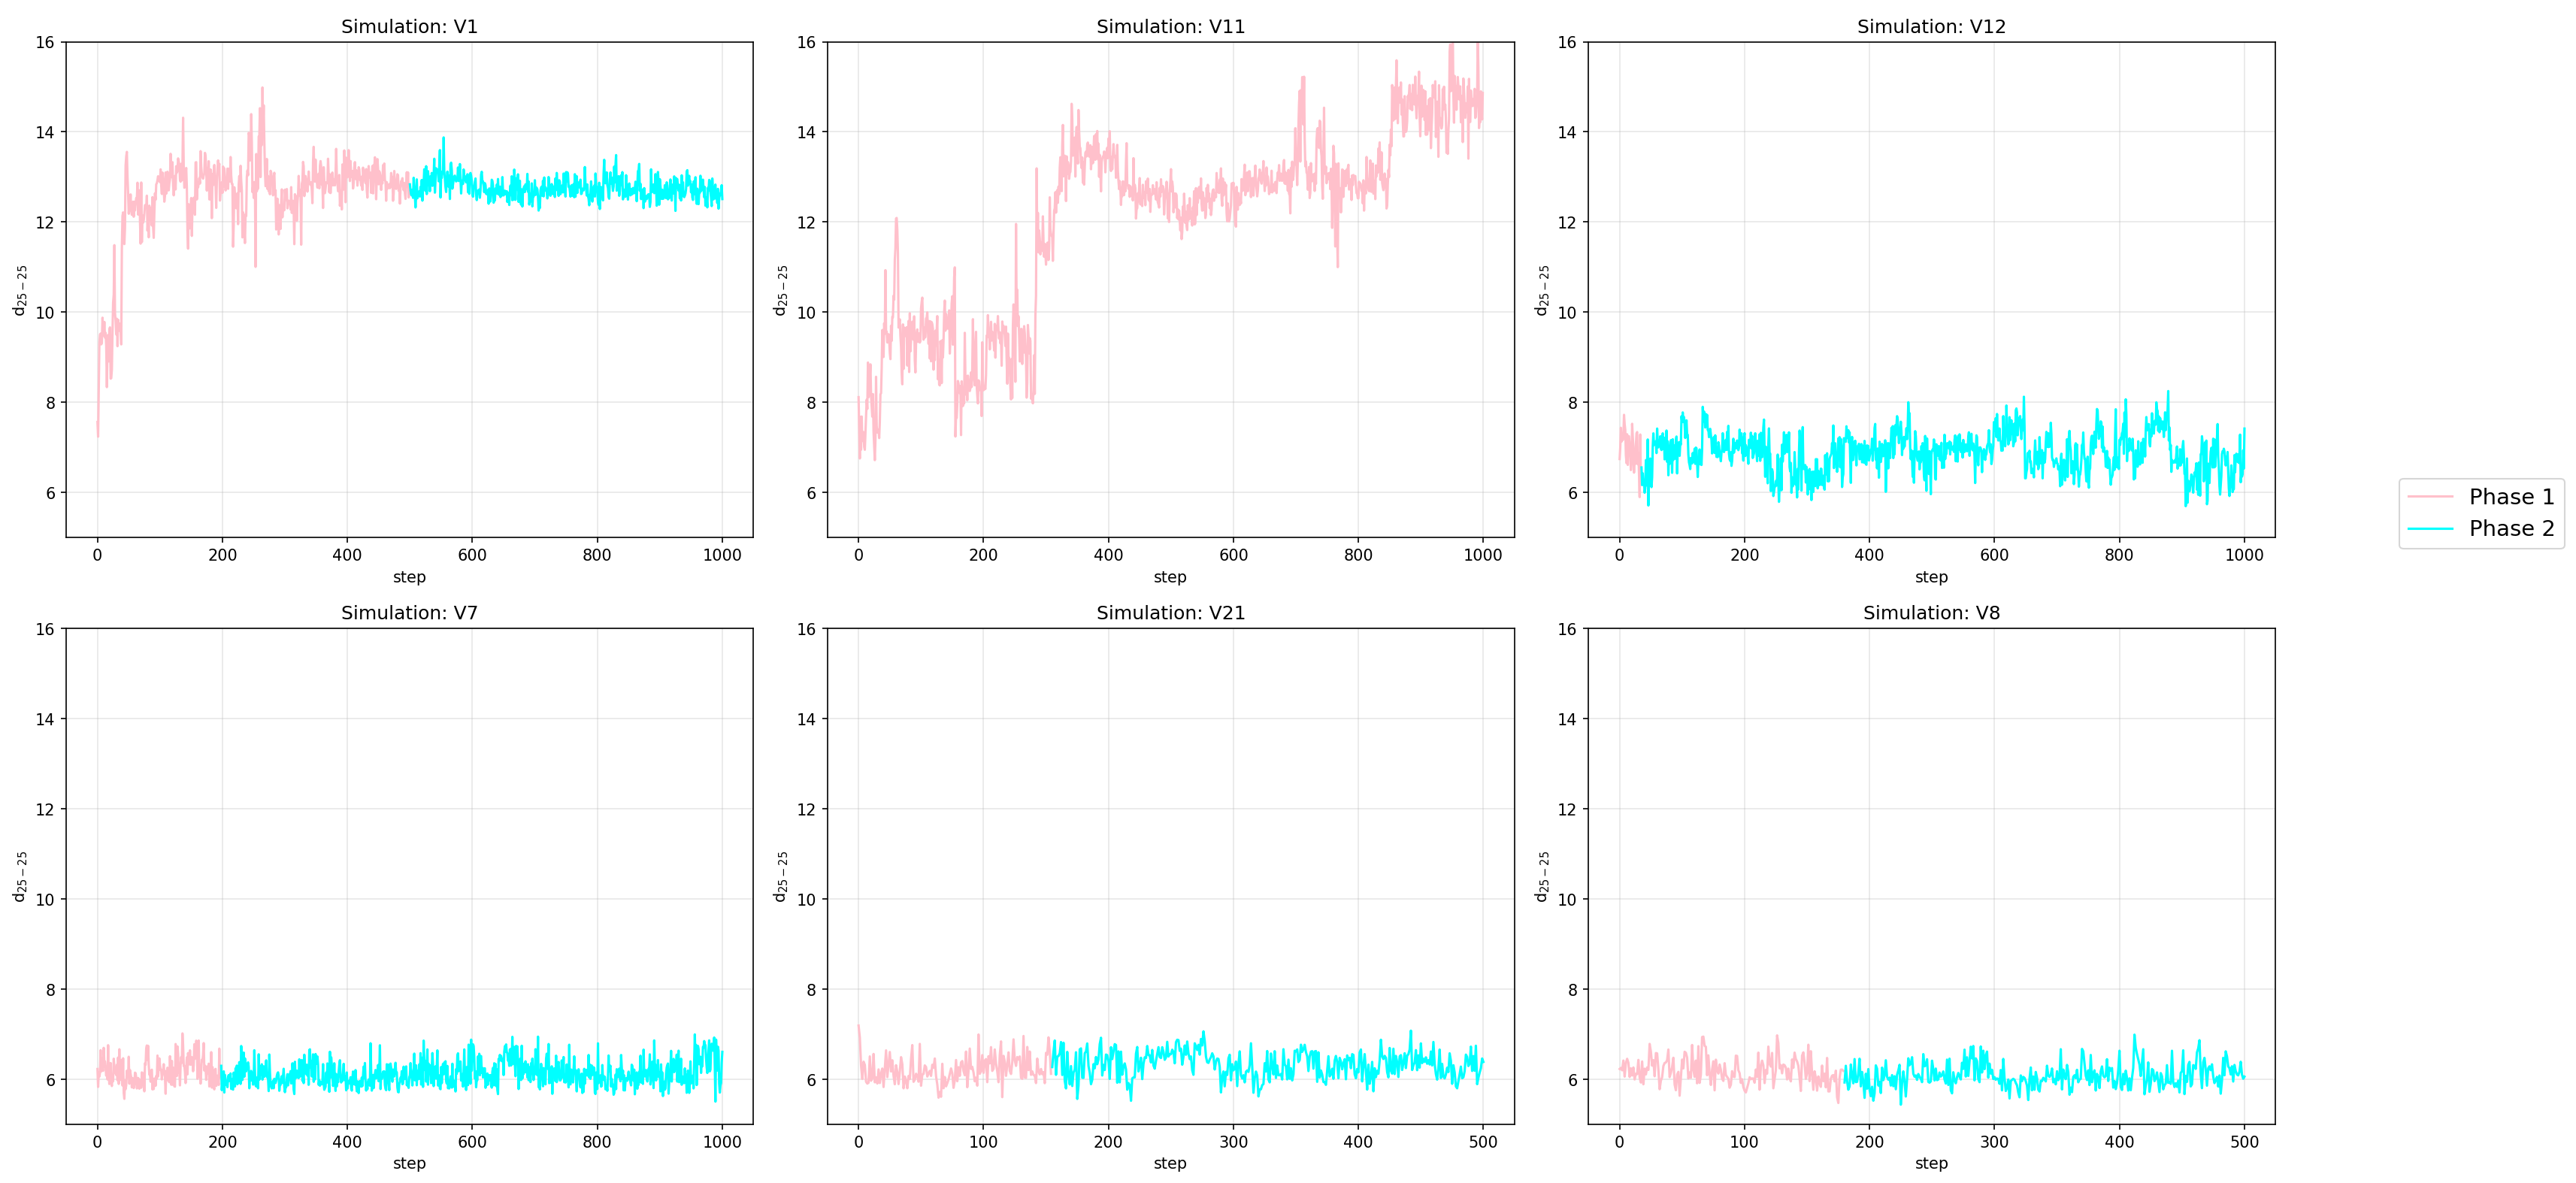
\includegraphics[width=\linewidth]{Figures/d_25_25.png}
		\caption{Analyse $d_{25-25}$ entre les dimères pour les six simulations : MP (V7,V8,V21) et DP (V1,V11,V12).}
		\label{fig:d25_25}
	\end{figure}
	
	\begin{figure}[h]
		\centering
		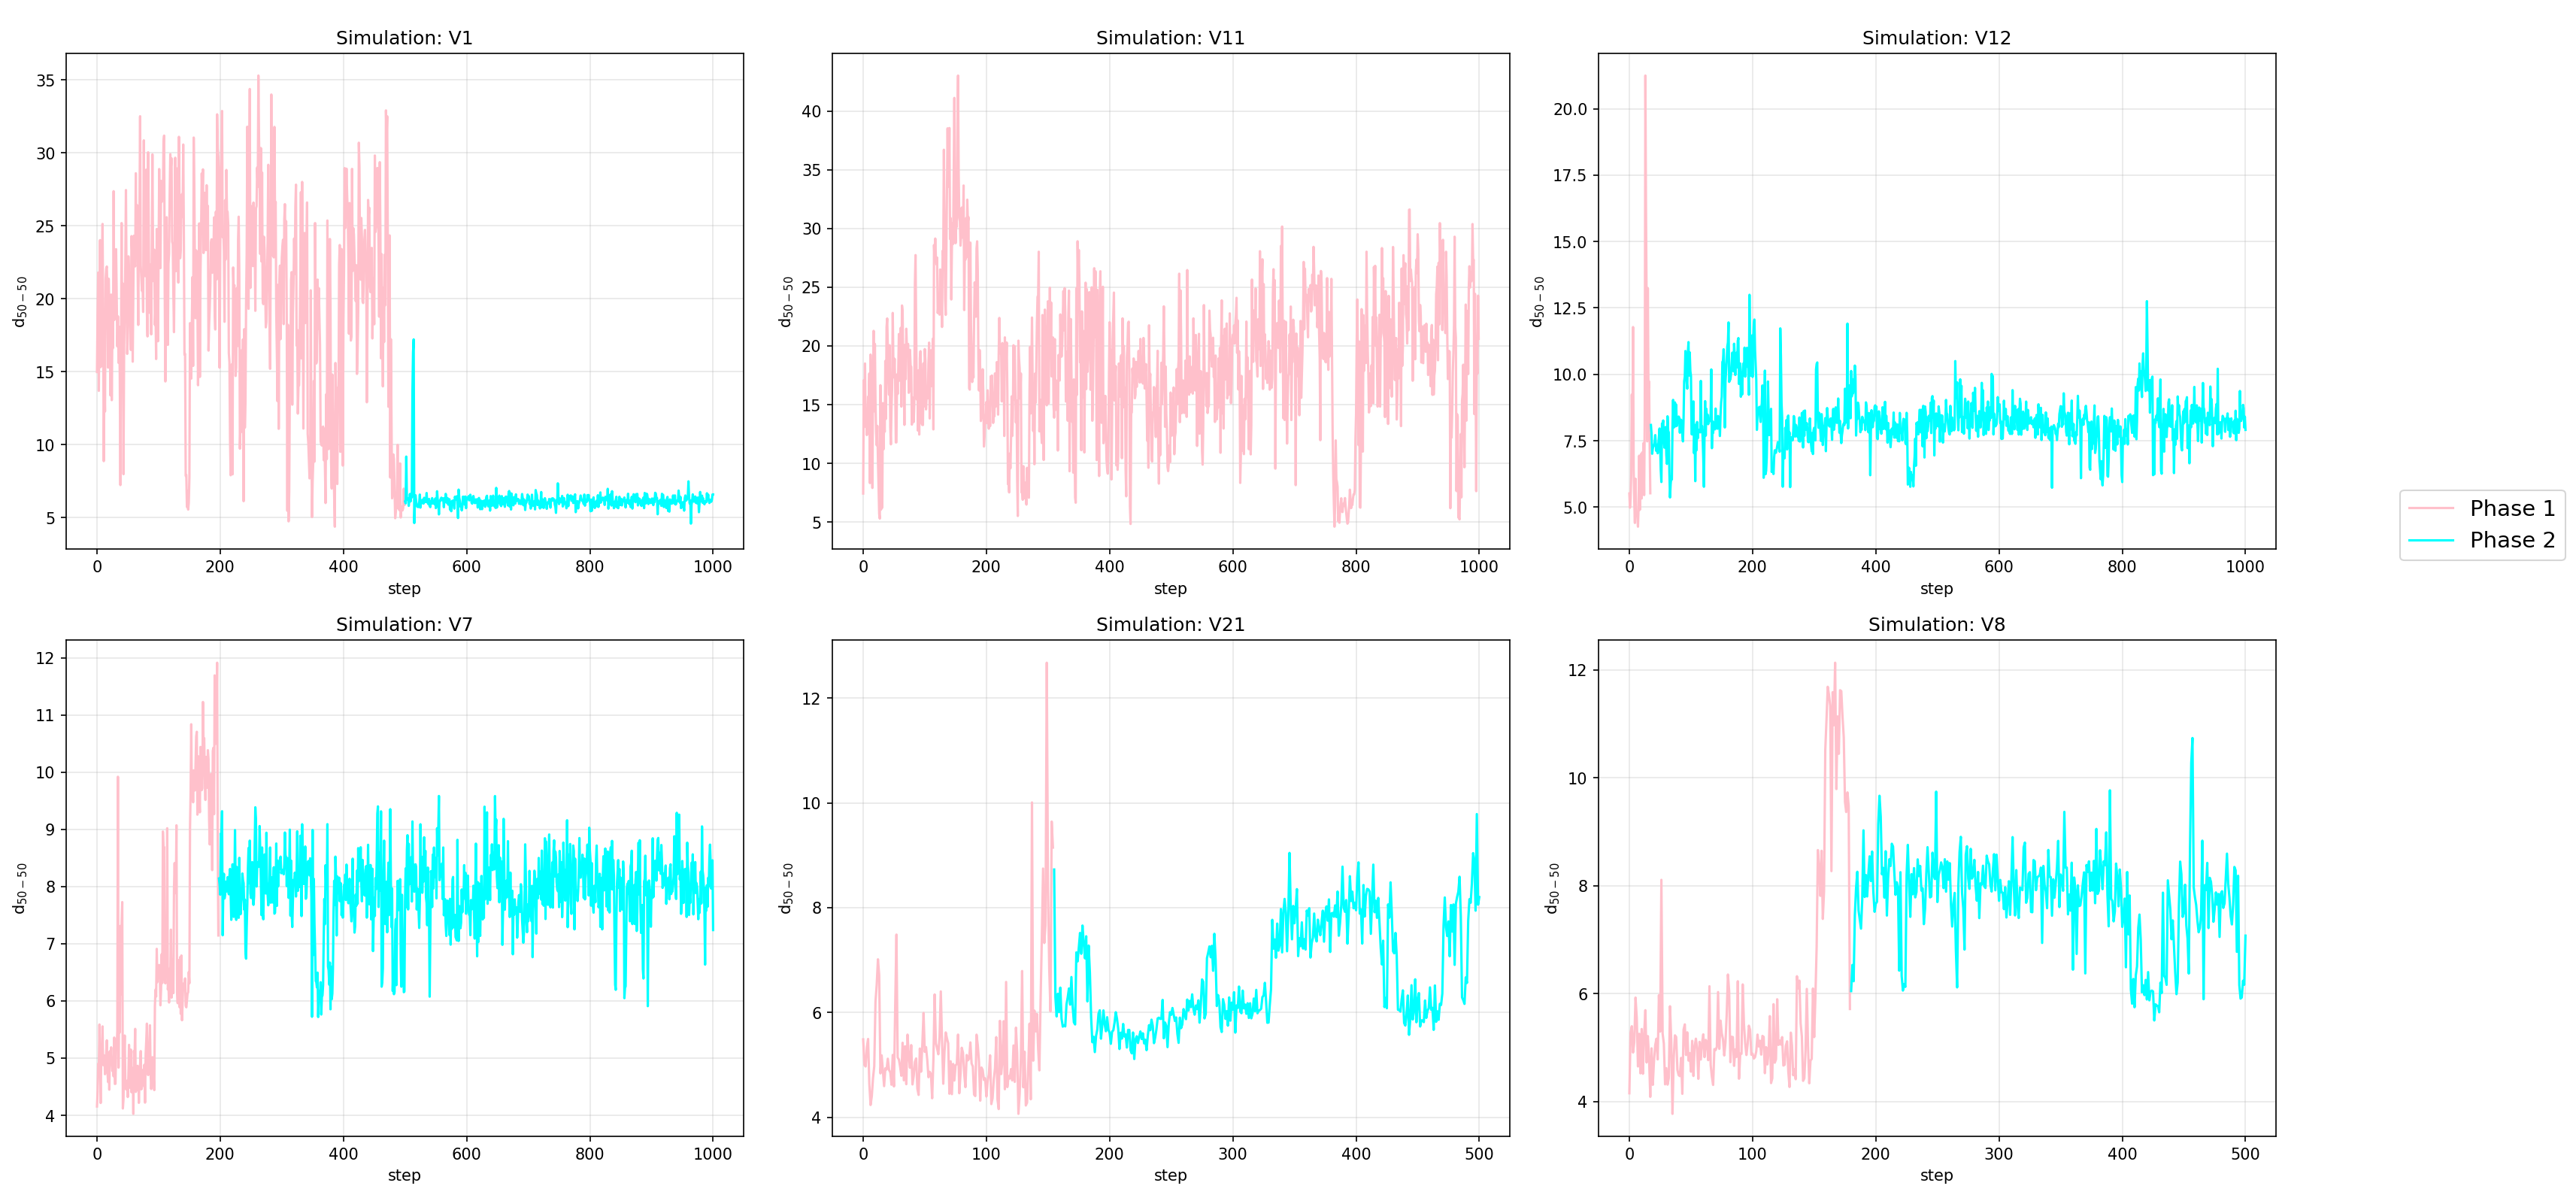
\includegraphics[width=\linewidth]{Figures/d_50.png}
		\caption{Analyse $d_{50-50}$ entre les dimères pour les six simulations : MP (V7,V8,V21) et DP (V1,V11,V12).}
		\label{fig:d50}
	\end{figure}

	\begin{figure}[h]
		\centering
		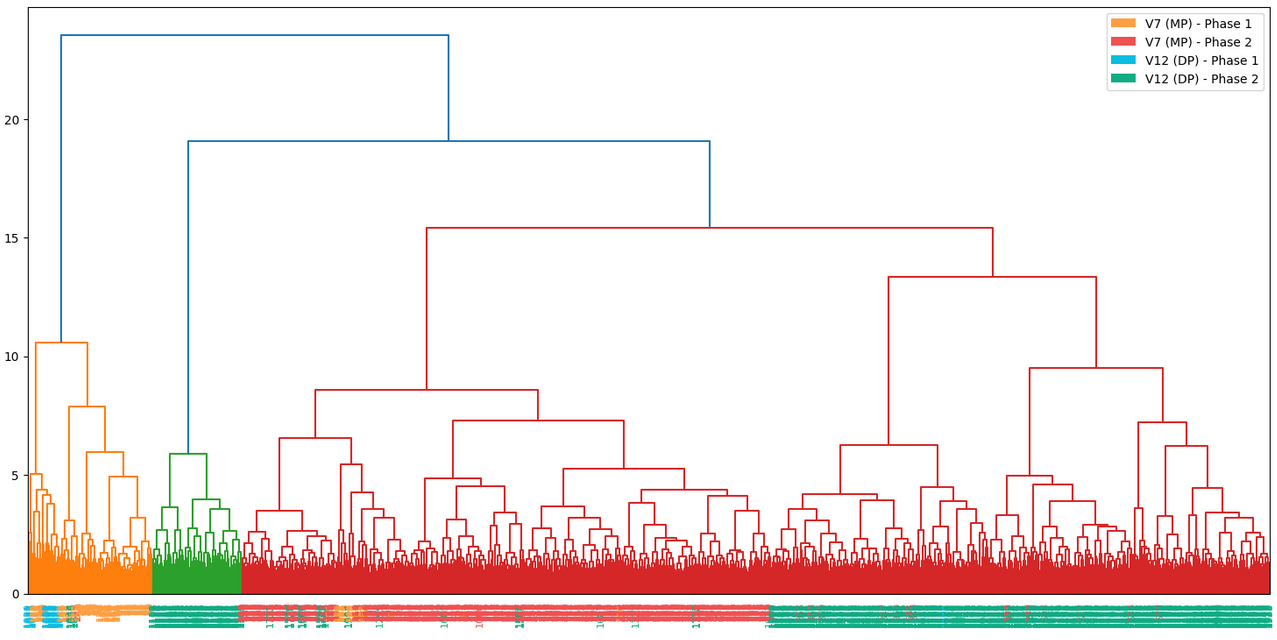
\includegraphics[width=\linewidth]{Figures/dendrogrammRMSD.png}
		\caption{Regroupement de frames individuels de V7 (MP) et V12 (DP) basé sur le $\text{RMSD}_{\text{pairs}}$ (méthode Ward).}
		\label{fig:dendro_RMSD}
	\end{figure}

	\begin{figure}[h]
		\centering
		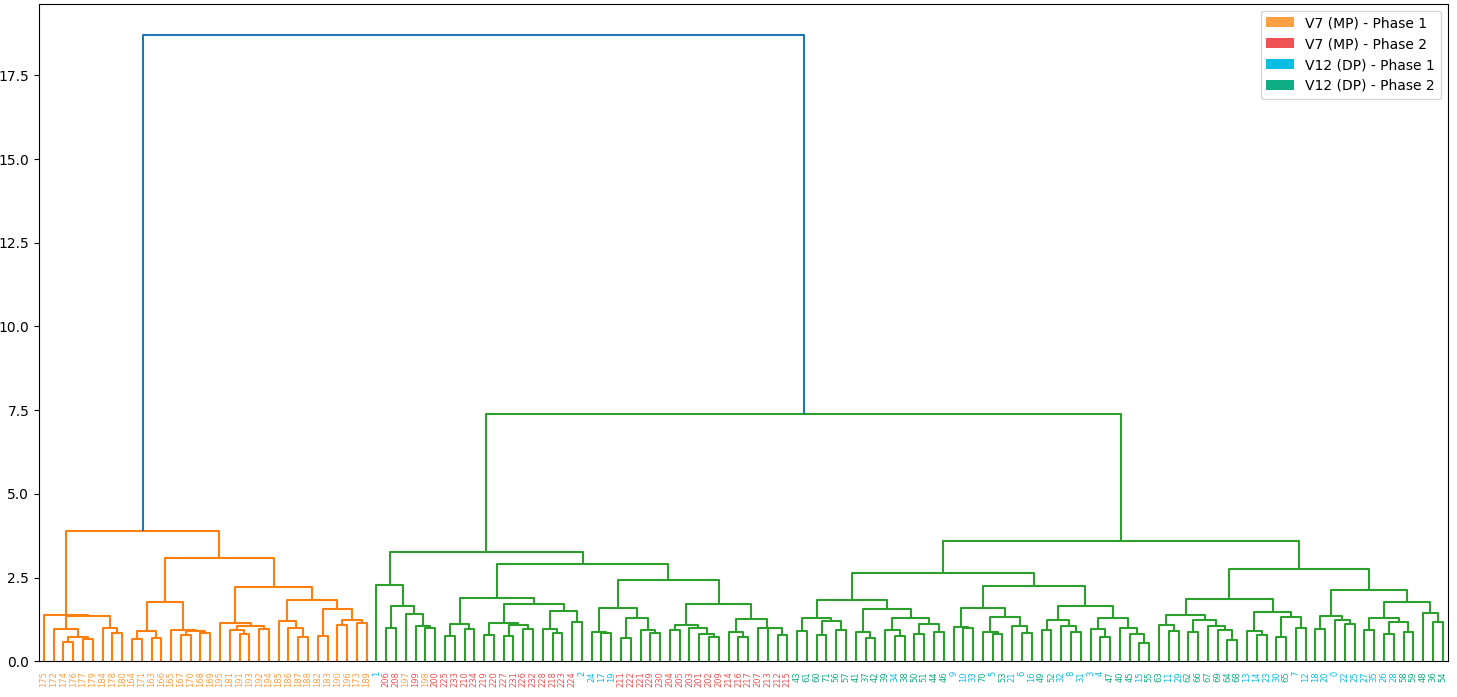
\includegraphics[width=\linewidth]{Figures/dendrogram_jaccard_sim.png}
		\caption{Regroupement de frames individuels de V7 (MP) et V12 (DP) au moment de transition entre deux phases ($\pm36~\text{ns}$) basé sur la distance de Jaccard (méthode Ward)}
		\label{fig:dendro_Jaccard}
	\end{figure}

	
	\cleardoublepage
	
\end{document}